%% ==================
\chapter{First results: Study of the excess}
\label{ch:results}
%% ==================
%
%My results:

\section{Recreating previous results}
\label{sec:results_recreating_prev_res}
%	-Only 3 original components
%		-Spherical excess
%		-very bad chi2 in disk and bubbles

%Introduce the weniger plots here (or in the state of the research?) to show excess in GC.
%\begin{figure}[h]
%  \centering
%  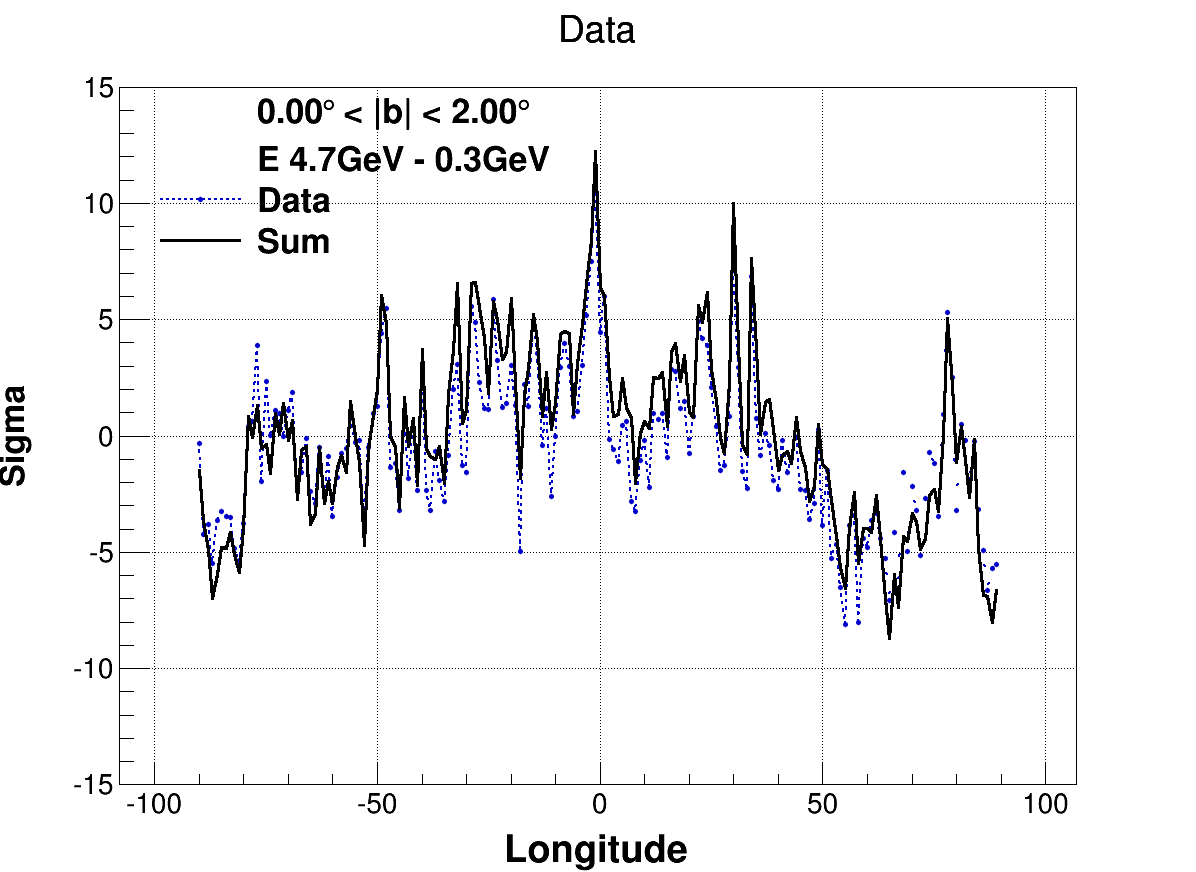
\includegraphics[width=.5\linewidth]{pic/results/Weniger_SUM_b0-2_E4,7-0,31GeV.png}
%  \caption{Some weniger plots to show the GC excess}
%  \label{fig:weniger_plot}
%\end{figure}


\begin{figure}[h]
  \centering
%  \begin{minipage}[h]{0.45\textwidth}
%  	\centering
%	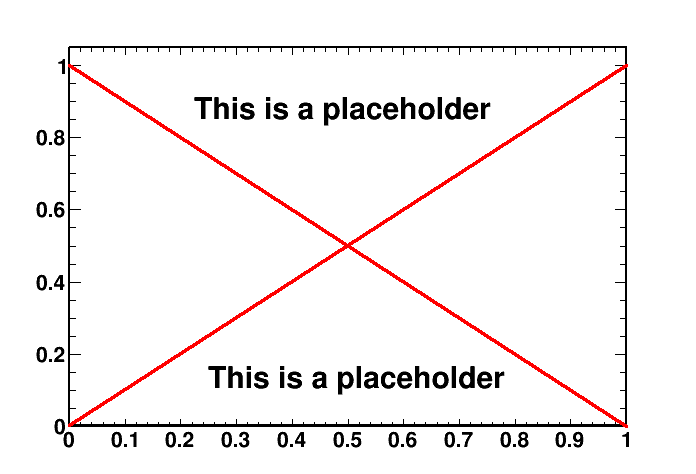
\includegraphics[width=1.\linewidth]{pic/dummy.png}
%  	\subcaption{Picture of GC excess as fitted previously (https://arxiv.org/pdf/1110.0006.pdf?)}
%  	\label{fig:original_GC_excess}
%  \end{minipage}
  \begin{minipage}[h]{0.45\textwidth}
  	\centering
	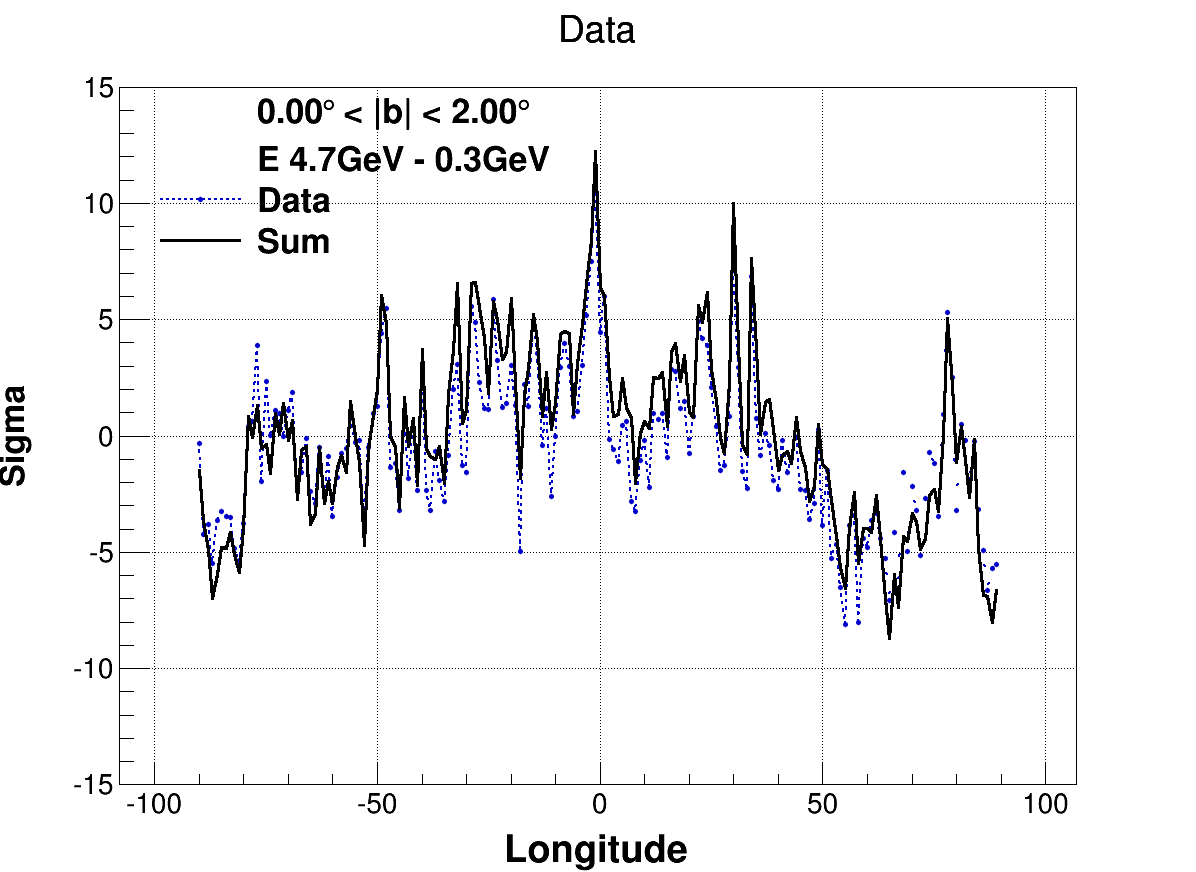
\includegraphics[width=1.\linewidth]{pic/results/Weniger_SUM_b0-2_E4,7-0,31GeV.png}
  	\subcaption{}
  	\label{fig:weniger_plot}
  \end{minipage}
  \hfill
  \begin{minipage}[h]{0.45\textwidth}
	  \centering
	  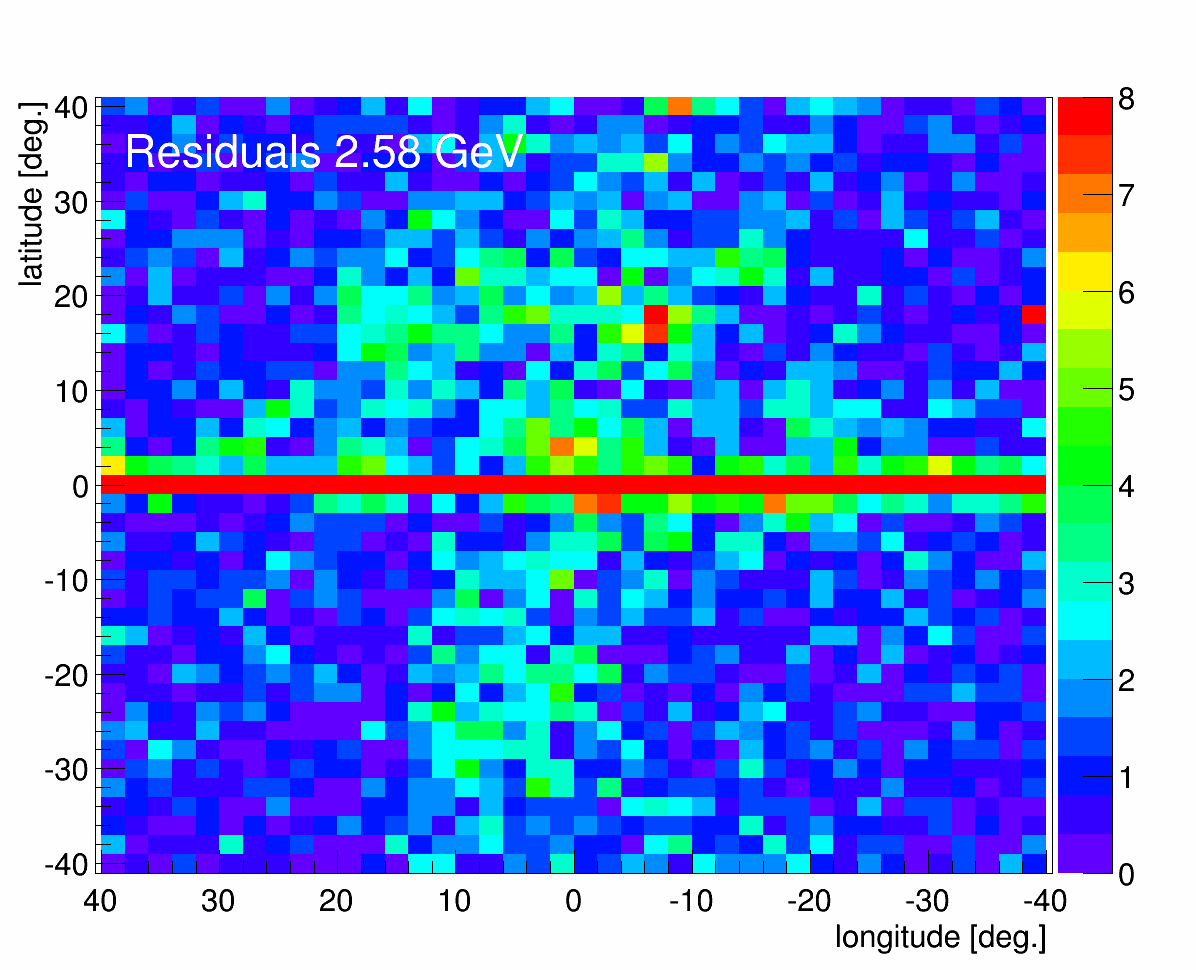
\includegraphics[width=1.\linewidth]{pic/results/BKGonly_halo_residuals.png}
	  \subcaption{}
	  \label{fig:our_excess}
  \end{minipage}
  \caption{Representation of the GC excess. (a) Approximation of the Fermi data index (in blue) between 4.7 and 0.3 GeV for all longitudes below 2 degrees in latitudes. The peak in the GC indicates a harder spectrum that could trace the excess. In comparison the fitted background model (in black) do not show the peak.  TODO{Show the model, but without the excess component!}. (b) Map around the GC of the difference  in percent between the model and the data at 2 GeV. The disk is very problematic, but the interesting feature is the more or less spherical shape around it. The difference decreases as the distance from the GC increases.}
  \label{fig:GC_excess}	 
\end{figure}

Before trying to upgrade the current model, it is important to make sure it can be recreated with this method. 

\ref{fig:weniger_plot} and \todo{ref Appendix with more weniger plots} illustrate a way of seeing the excess, without using any fit method, only the data. For absolute latitudes below two degrees, an approximation of the index of the Fermi data spectrum between 5 GeV and 300 MeV is plotted for all longitudes. For every sky direction, $\sigma$ is given by equation ref where error is the cumulated uncertainty on both data points.
\begin{equation}
\sigma = \frac{\left(Data(l, b, E_1) - Data(l, b, E_2) \right)}{\sqrt{\sigma_{1,\ stat}^2 + \sigma_{2, stat}^2}}
\end{equation}


It is then rescaled around zero for visibility. A peak is dominating in the center, indicating an increase in the spectrum index. This can be interpreted as the excess component rising and changing the shape of the spectrum.

Fig. \ref{fig:our_excess} present an other way of looking at the excess with a fit using only the background components (PCR, IC and BR). This map shows the percentage difference between the fit and the data at 2.58 GeV. This gives an idea about the distribution of the excess around the GC. The shape and intensity of the previously observed excess are found \todo{cite https://arxiv.org/pdf/1110.0006.pdf? or others}. Excluding the galactic disk for latitudes below two degrees, the excess extends to $30^\circ$ in all directions from the GC.The problem only confirm itself when looking deeper into the results.


\begin{figure}[h]
  \centering
  \begin{minipage}[h]{0.45\textwidth}
  	\centering
	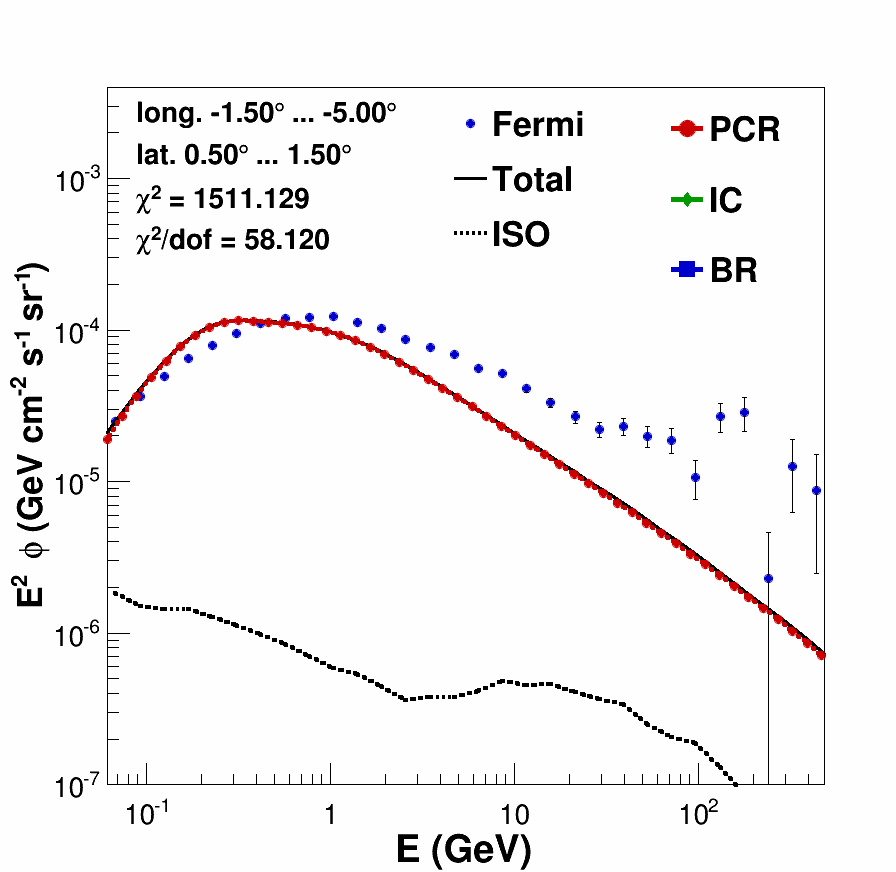
\includegraphics[width=1.\linewidth]{pic/results/BKGonly_CMZ.png}
  	\subcaption{}
  	\label{fig:bkgd_only_spectrum}
  \end{minipage}
  \hfill
  \begin{minipage}[h]{0.45\textwidth}
	  \centering
	  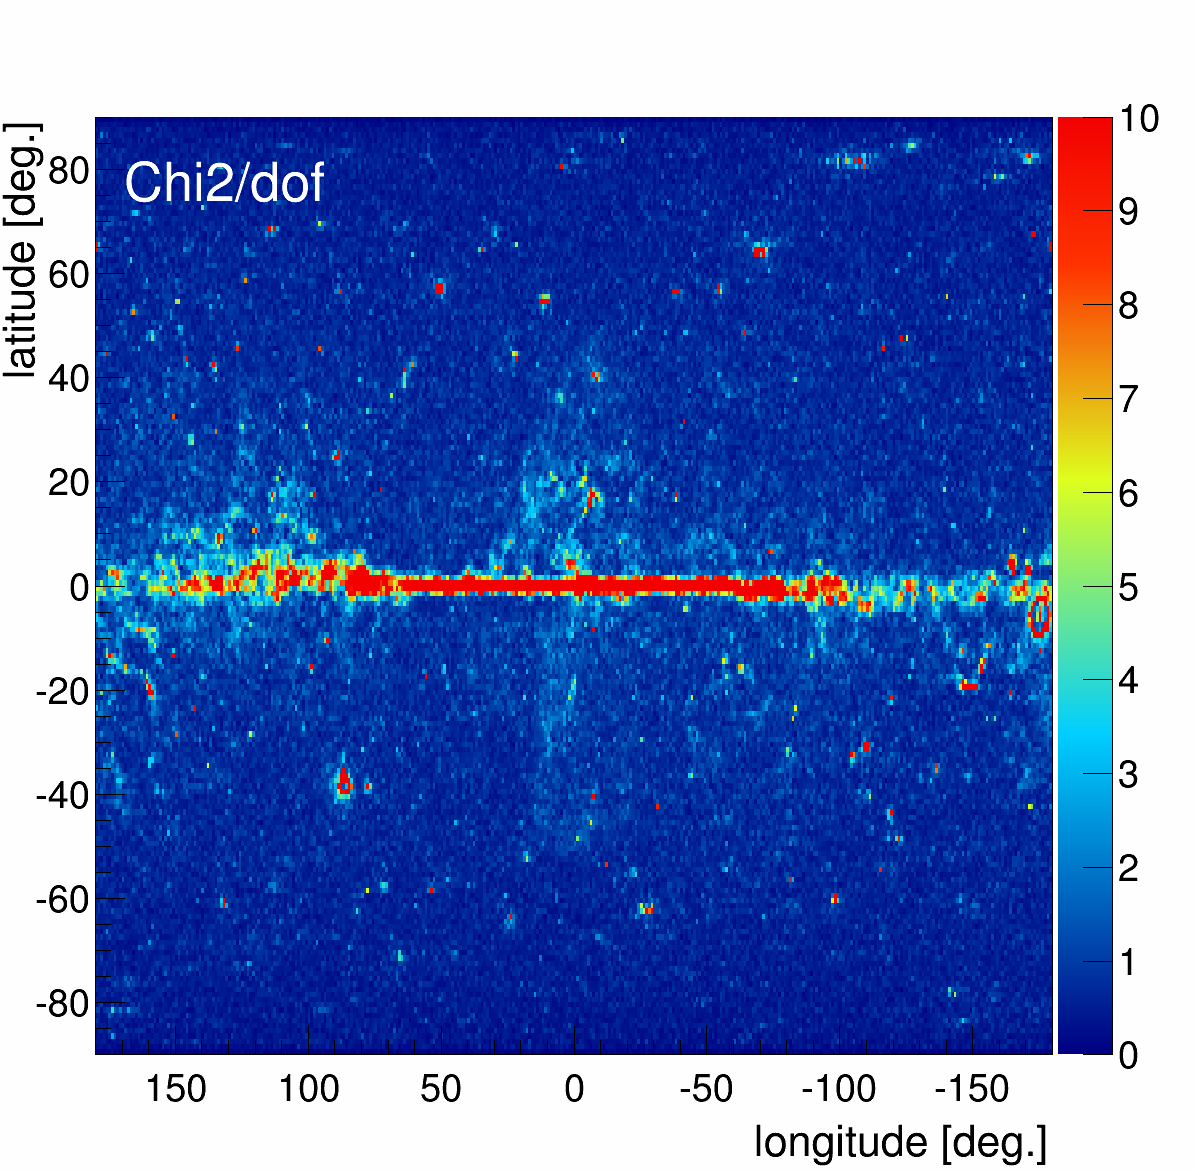
\includegraphics[width=1.\linewidth]{pic/results/BKGonly_fine_chi2_distribution.png}
	  \subcaption{}
	  \label{fig:BKGonly_chi2Distribution}
  \end{minipage}
  \caption{(a) Spectrum of the CMZ region and its fit using only the three background components. Two major problems can be identified. First a hardening of the spectrum above 10 GeV; second the shift of the spectrum maximum between the model and the Fermi data. (b) The best $\chi^2$ value obtained by the fit for every sky direction. The bubbles structures and the galactic disk are visible, with a very large disagreement between the model and the data. These bad $\chi^2$ regions are the sign that one or two of the problems identified on the left are present. Several bad spots can also be identified. These correspond to a bad point source subtraction when processing the data (cf. chapter \ref{ch:method}) and should be ignored.}
  \label{}
\end{figure}


Looking at the $\chi^2$ distribution on the sky (Fig. \ref{fig:BKGonly_chi2Distribution}), the bubbles and the disk appear clearly in red, showing a high $\chi^2$ value. The fit does not give proper results in those regions, with the high energy part of the spectrum not described by the three background templates as shown by Figure \ref{fig:bkgd_only_spectrum}. This example spectrum from the galactic center illustrates the two main problems. First, the high energy tail of the data is not compatible with the model, much higher and with a harder spectral index. The second problem is the shift in the peak position. The data peaks around one or two GeV when the model peaks only around a few hundred MeV. These two differences shall be investigated in more detail in the following sections.
But outside these regions, the fit works a lot better, with a $\chi^2$ not much bigger than three. This is not perfect, but in comparison with the disk, it is undeniably an improvement.


%where the high energy spectrum is harder (see Fig. \ref{fig:bkgd_only_spectrum}). In this region, the PCR spectrum falls off too quickly, and the IC spectrum which usually takes care of high energies is blocked by the low energy flux drop.

\subsection{EGRET Data}

One of the previous gamma-ray space telescope called the Energetic Gamma Ray Experiment Telescope (EGRET) gave a first insight on the GC excess. Its energy range did not exceed 30 GeV, and the data overall quality is worse than the LAT. But it is a good way to compare the results. A model for DM was fitted on the EGRET data to test the hypothesis. Figure \ref{fig:EGRET_comp_a} and \ref{fig:EGRET_comp_b} compares the results of this study to the EGRET study. For a large region around the GC, the Fermi and EGRET data were fitted with a PCR, IC, BR and DM template. The WIMP mass is 40 GeV and the fit only considers points below 10 GeV, even if it shows the higher energies as well, to be consistent for both study. It is a first attempt to recreate previous results with an excess component.
When the fit works perfectly for the EGRET data on the left, a clear deficit can be observed for Fermi data. Above 10 GeV, EGRET has no data and the shape could lead to believe that a rapid drop occurs. But Fermi does not show this drop, and present a harder spectrum than what could be expected from EGRET data. The difference is all in this hard high energy tail. It shows that even if the first measurements could be fitted by adding a single excess component like DM, it is not possible with Fermi data: the addition of a new component with a very hard spectrum is necessary. This is done in the next section, with the introduction of the SCR component.

\begin{figure}[h]
  \centering
  \begin{minipage}[h]{0.45\textwidth}
  	\centering
	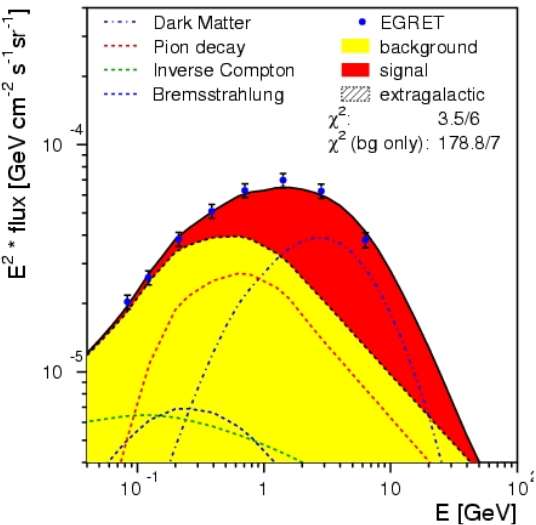
\includegraphics[width=\linewidth, height=5.6cm]{pic/results/EGRET_A.png}
	\subcaption{EGRET}
  	\label{fig:EGRET_comp_a}
  \end{minipage}
  \hfill  
  \begin{minipage}[h]{0.45\textwidth}
  	\centering
	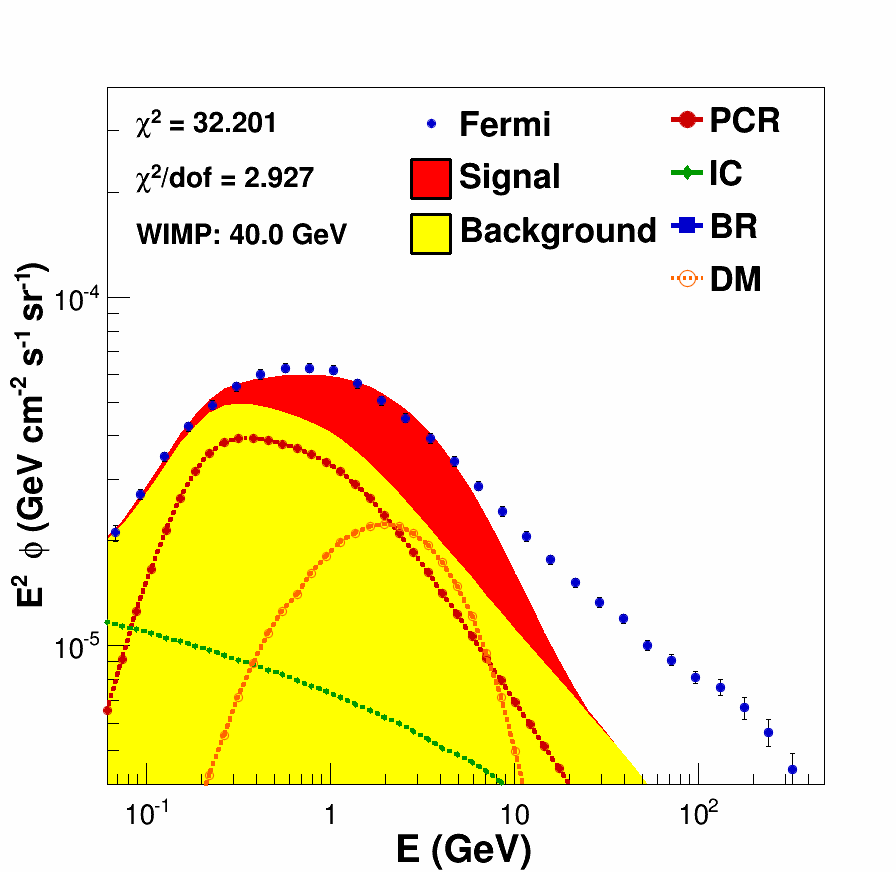
\includegraphics[width=1.\linewidth]{pic/results/asEGRET_Fermi_A.png}
  	\subcaption{Fermi}
  	\label{fig:EGRET_comp_b}
  \end{minipage}
%  \hfill  
%  \begin{minipage}[h]{0.3\textwidth}
%  	\centering
%	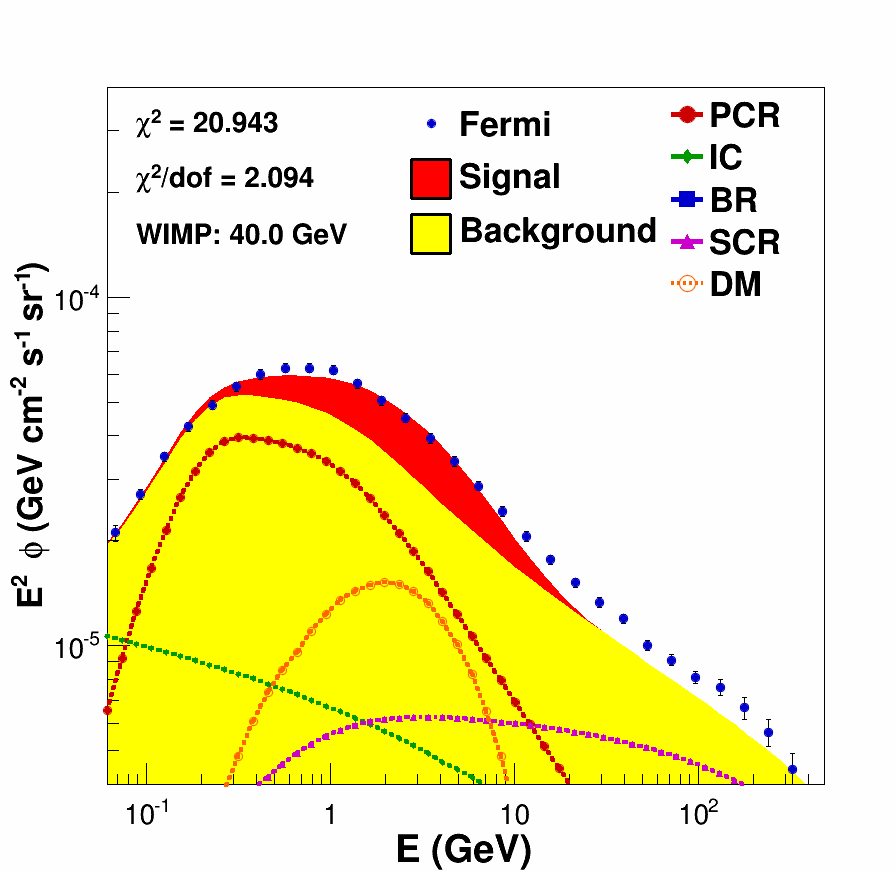
\includegraphics[width=1.\linewidth]{pic/results/asEGRET_SCR_Fermi_A.png}
%  	\subcaption{Fermi with SCR component}
%  	\label{fig:EGRET_comp_c}
%  \end{minipage}
  \caption{Comparison of the EGRET (a) and Fermi (b) data with the model. The EGRET data were fitted by cite{EGRET paper}, and their model take a PCR, BR, IC and dark matter templates. The maximum energy of the EGRET data is 10 GeV, and the model agrees relatively well at all energies. The model used on the Fermi data is as close as possible from the EGRET model, with the PCR, BR, IC and DM template of this study, but this time the data go up to 500 GeV. Once again, the model agrees for all energies below 10 GeV; but it can not account for the energies above. This is an indication that high energies are harder than expected and require the addition of a new component to the model.}
  \label{fig:EGRET_comp}
\end{figure}

%I was able to recreate a more or less spherical excess in GC around 2GeV.\\
%Bad fit in disk and bubbles as expected.
%Two problems :
%\begin{itemize}
%\item Spectrum too hard at high energies
%\item Excess around 2GeV
%\end{itemize}

\newpage
\section{Introducing SCR}

\begin{figure}[h]
  \centering
  \begin{minipage}[h]{0.45\textwidth}
  	\centering
	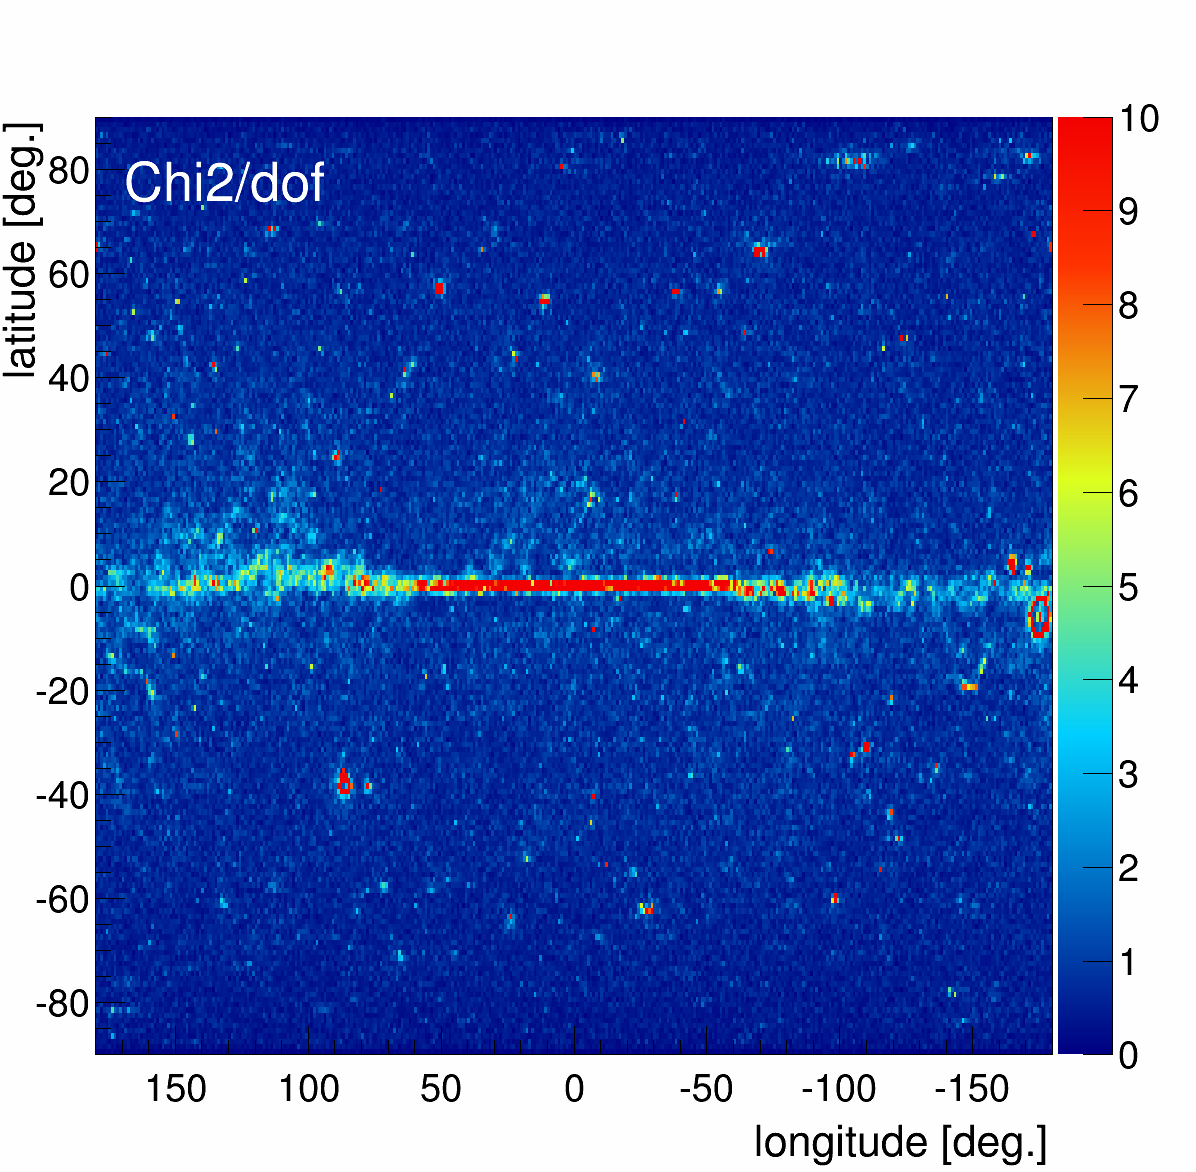
\includegraphics[width=1.\linewidth]{pic/results/SCRonly_fine_chi2_distribution.png}
  	\subcaption{Chi2 distribution of SCR only fits.}
  	\label{fig:SCRonly_fit}
  \end{minipage}
  \hfill
  \begin{minipage}[h]{0.45\textwidth}
	  \centering
	  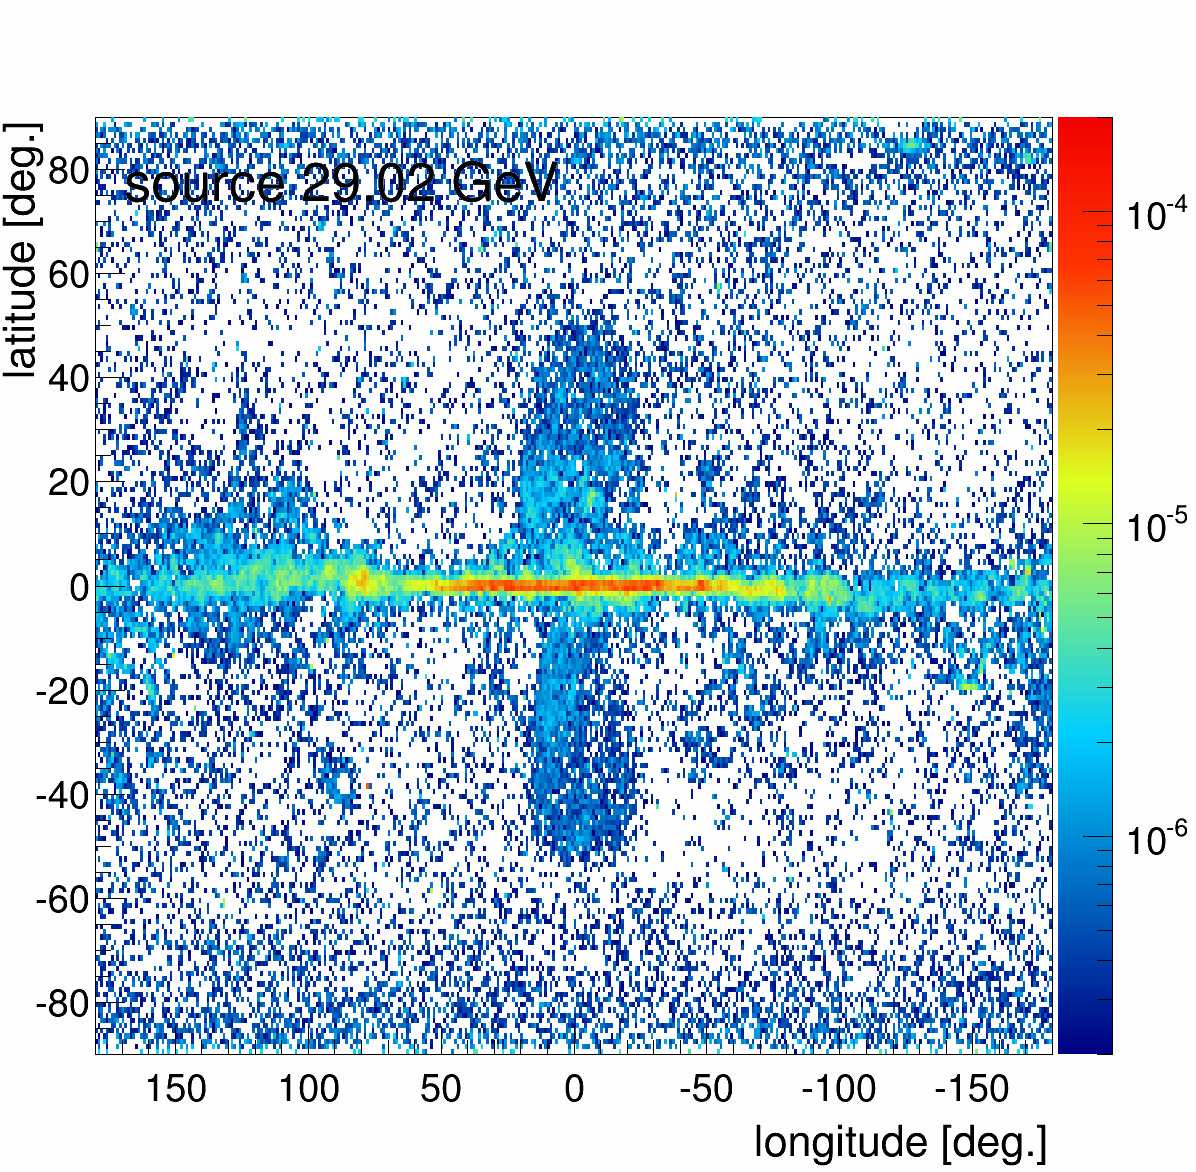
\includegraphics[width=1.\linewidth]{pic/results/SCRonly_fine_SCR_distribution_E20.png}
	  \subcaption{Flux distribution of SCR only fits.}
	  \label{fig:BKGonly_bubble_spec}
  \end{minipage}
  \caption{Results of fit including the SCR component. (a) $\chi^2$ distribution. The bubbles are not so clear than before, but the disk is still visible (cf Fig. \ref{fig:BKGonly_chi2Distribution}). (b) Flux distribution of the SCR template at 30 GeV. The bubbles and the disk are distinct. The SCR template traces the hardening in the data high energy spectrum, thus showing it here. This distribution was expected, in the bubbles because of unpropagated proton CR ejected from the GC, and in the disk because of point sources that are not subtracted.}
  \label{fig:SCRonly_distributions}
\end{figure}


As seen previously, a fourth component is needed to fit the data in the disk and the bubbles in addition to the basic templates. This is due to a hardening of the spectrum at high energy that is thought to be induced by non propagated CR, i.e. CR that do not propagate through dense gas clouds or highly convoluted magnetic fields. For example in the bubbles, where particles are ejected without passing through dust clouds; or simply near sources, where CR do not have time to interact with the interstellar medium.


After introducing the SCR template, a clear improvement can be noted in the $\chi^2$ distribution (comparing Fig. \ref{fig:SCRonly_fit} to Fig. \ref{fig:BKGonly_chi2Distribution}). The bubble shape that was delimited before by a bad $\chi^2$ zone has now disappeared. Even if the fit is still not perfect everywhere, the improvement is significant.
The disk is still not fitted properly, with very high $\chi^2$ values. Some structures can also be seen along the disk for absolute longitudes over $90\circ$. These remaining bad fits tends to show that the model is still not optimal yet, and could be improved, as seen in following sections.

\begin{figure}[h]
  \centering
  \begin{minipage}[h]{0.45\textwidth}
  	\centering
	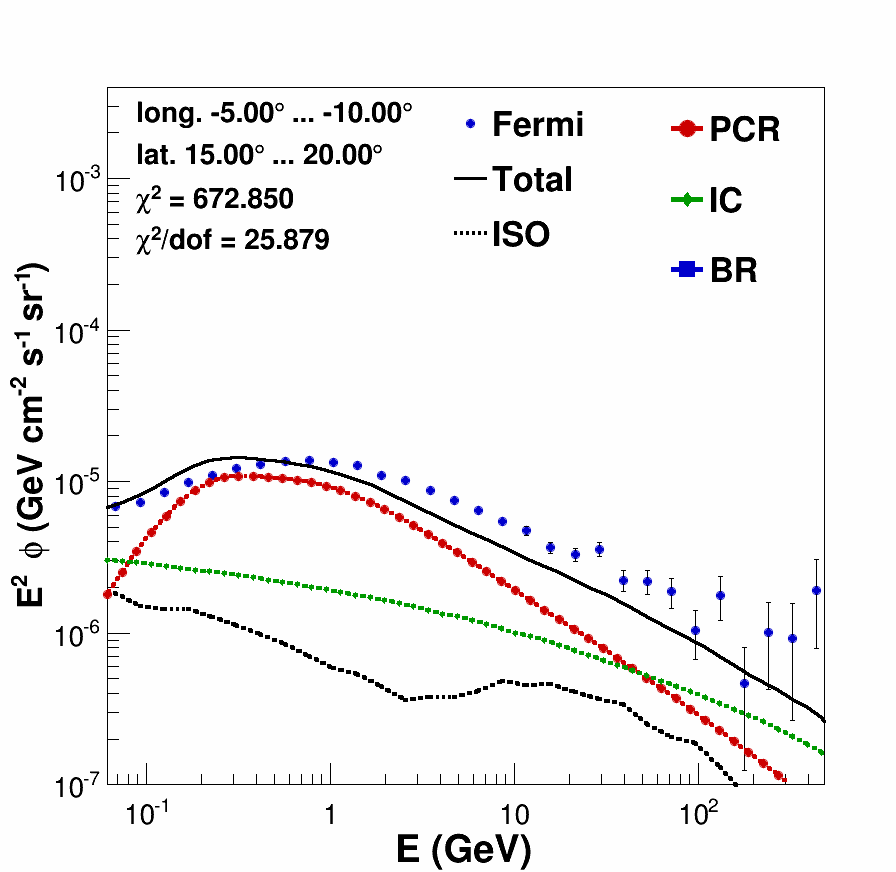
\includegraphics[width=1.\linewidth]{pic/results/bkgdonly_spectra_bubble_example.png}
  	\subcaption{}
  	\label{fig:SCRonly_bubble_spec}
  \end{minipage}
  \hfill
  \begin{minipage}[h]{0.45\textwidth}
	  \centering
	  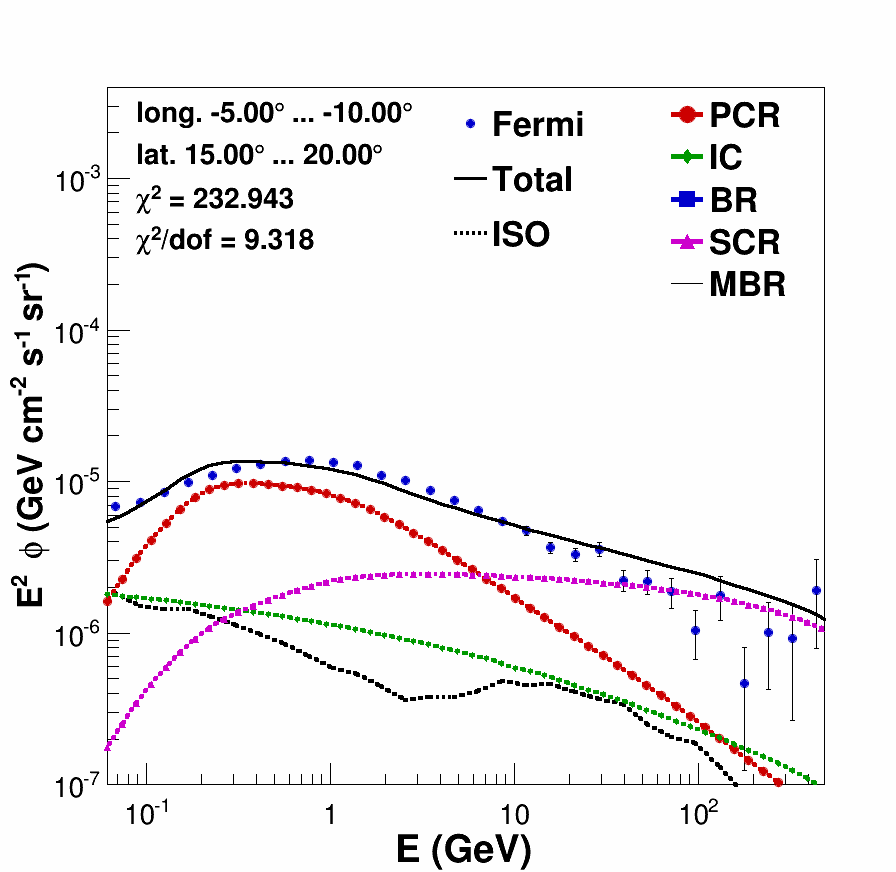
\includegraphics[width=1.\linewidth]{pic/results/SCRonly_spectra_bubble_example.png}
	  \subcaption{}
	  \label{fig:BKGonly_bubble_spec}
  \end{minipage}	 
  \caption{(a) Fit results in the direction of a bubble using only the three background templates. The problems identified before are here, with a hard high energy tail and a slight shift in the maximum position. (b) Fit results in the direction of a bubble using only the three background and the SCR template. This time, the small shift is still present, but the high energy hardening is fitted by the SCR template.}
	  \label{fig:SCRonly_BKGonly_spec_comp}
\end{figure}

The SCR template is present only in the disk and the bubbles (see Fig. \ref{fig:SCRonly_distributions}), as expected. The map of fitted SCR component shows it clearly, delimiting the bubbles with great precision. This distribution reinforces the idea of a source component, by pointing to all the regions where a hardening of the spectrum is present, as expected from its physical interpretation.
It also does not disrupt the other components distribution too much. The PCR, IC and BR distributions are similar and still match their expected shape. \todo{add Appendix skymaps of all components for noSCR and SCR, to compare}.

Figure \ref{fig:SCRonly_BKGonly_spec_comp} shows the spectrum in a given direction inside the bubbles, before and after adding the SCR template. While the high energy parts (above 100 GeV) of the spectra are dominated by SCR, the lower energies are also fitted with PCR and IC. The major difference is that each template fit one part of the spectrum, leaving other component deal with the rest. SCR is present at high energies, and this leaves more room for PCR and IC to adapt to the low energy spectrum. Hence increasing the fit quality.



\begin{figure}[h]
	\centering
	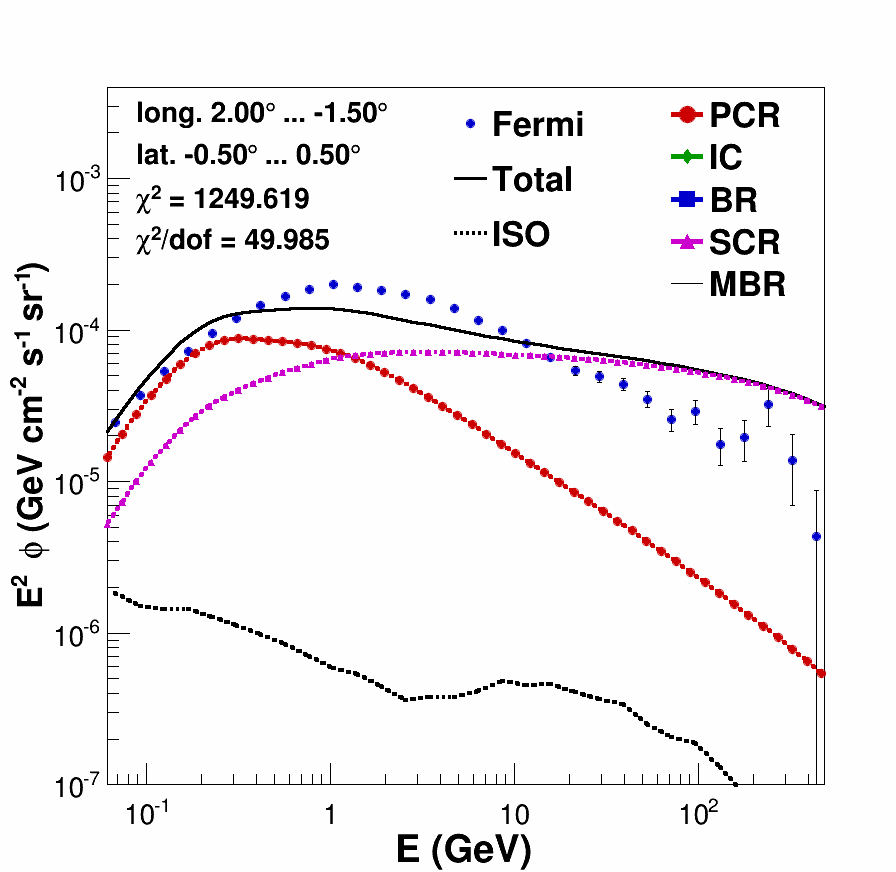
\includegraphics[width=.5\linewidth]{pic/results/SCRonly_CMZ.png}
	\caption{Spectrum from the GC, where the excess is supposed to be the highest. The SCR component overshoot the high energies to compensate a lack of gamma ray flux at 2 GeV. But introducing an excess component should cover the lack and the SCR contribution should decrease everywhere the 2 GeV excess is present.}
	\label{fig:SCRonly_CMZ_spec}
\end{figure}

This four-template fit represent a clear improvement compared to the background only (PCR, IC and BR) model. But, as seen on the $\chi^2$ distribution map, the disk and low latitudes regions are still not fitted properly. Figure \ref{fig:SCRonly_CMZ_spec} shows it well. The PCR spectrum does not peak at the right energy. The Fermi data has its maximum around a few GeV, while PCR's is only at a few hundred MeV. This problem leads to a very high contribution of SCR, trying to fit the data's maximum and the high energies at the same time; task that can not be done with SCR's spectral shape.
This leads to the introduction of the first excess component, added to solve this problem.




%From Fig. \ref{fig:SCRonly_bubble_spec} and \ref{fig:SCRonly_bubble_spec} we see the role of the SCR template at high energies, taking care of the high flux. It also permits a better fit of low energies by PCR and IC since they do not have to be everywhere at the same time.

%\todo{Here the bad chi2 comes from 0.1GeV region, where the PCR template does not fit the data. not from the 2GeV excess.}
%A problem still remains in the disk and diffuse regions around the galactic anticenter. 


\newpage
\section{Introducing SCR and MCR}
%	-Introduction of SCR and MCR
%		-very good chi2 in disk and bubbles
%		-spatial shapes of comps
%			-IC sperical (as expected) but depletion in disk
%			-BR low in bubbles replaces IC in disk
%			-PCR OK but low in disk
%			-MCR follows CO map, take place of PCR in disk
%			-SCR follows bubble structure

%\begin{figure}[h]
%  \centering
%%   \todo{May have to change it if we change the bckground model} 
%  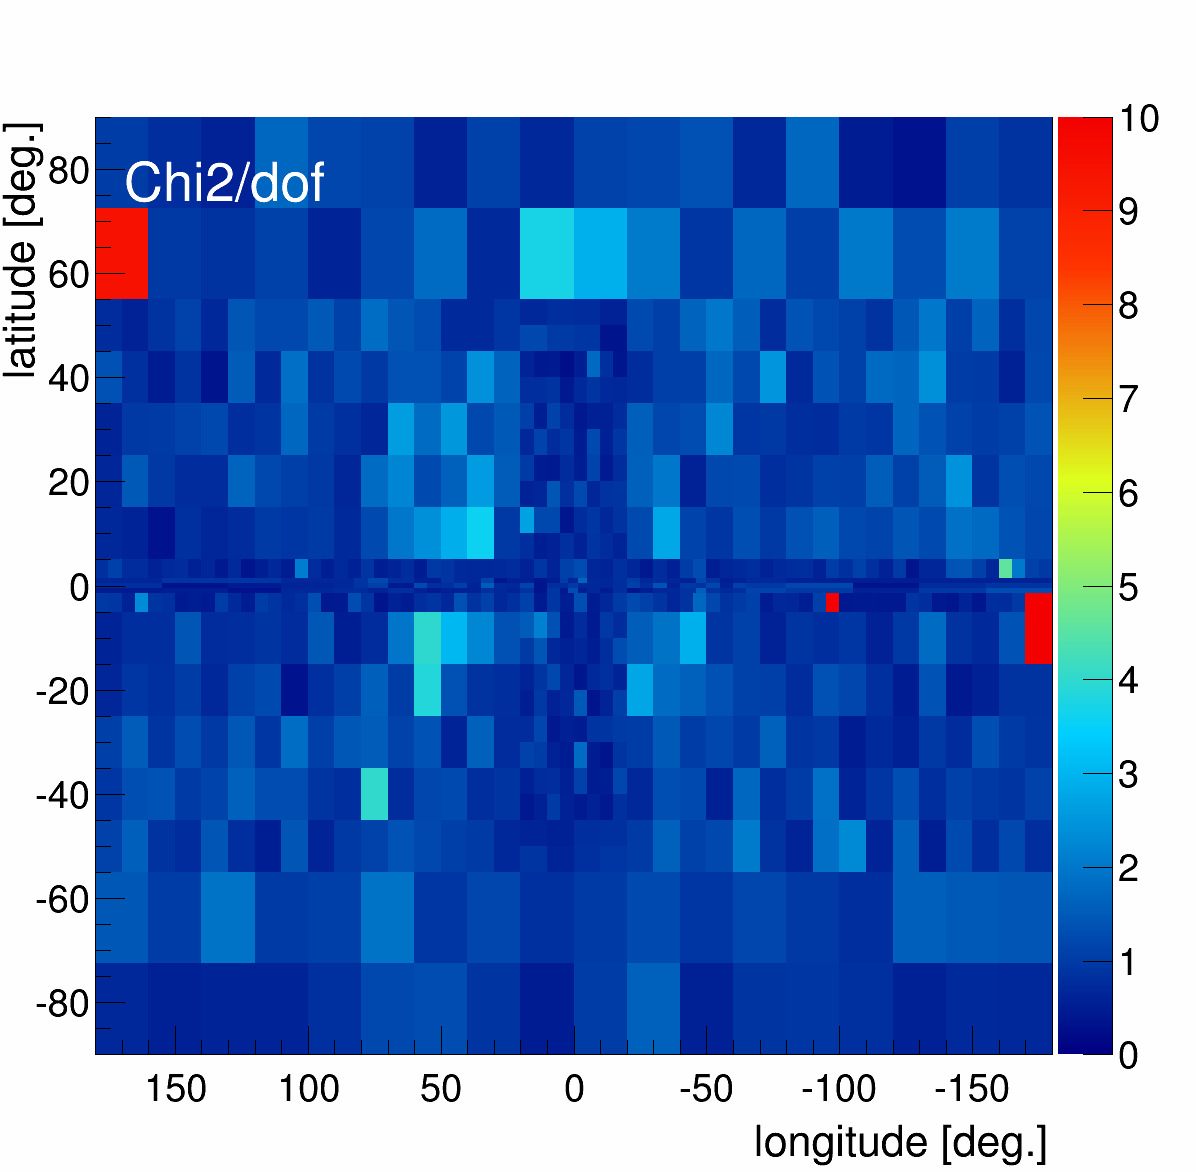
\includegraphics[width=.5\linewidth]{pic/results/MCRonly_chi2Distribution.png}
%  \caption{Chi2 maps of MCRonly fits compared to background only}
%  \label{fig:MCRonly_chi2Distribution}
%\end{figure}
%First obvious thing is the good chi2 in the disk and bubbles.\\

As shown on Fig. \ref{fig:MCRonly_chi2Distribution}, the addition of the new MCR template improves significantly the $\chi^2$ distribution in all directions. The bubbles and the disk structures are not visible any more. Such a flat distribution is one of the best indicator of a good fit.
Three red dots appear to have a really high $\chi^2$, but that is only due to the point source subtraction that is not perfect (see Chapter \ref{sec:Data_origin}). This direction can be identified on almost every fit done in this paper, and should not be taken into account too seriously for the analysis.

\begin{figure}[h]
  \centering
%  \begin{minipage}[h]{0.45\textwidth}
%	  \centering
%	  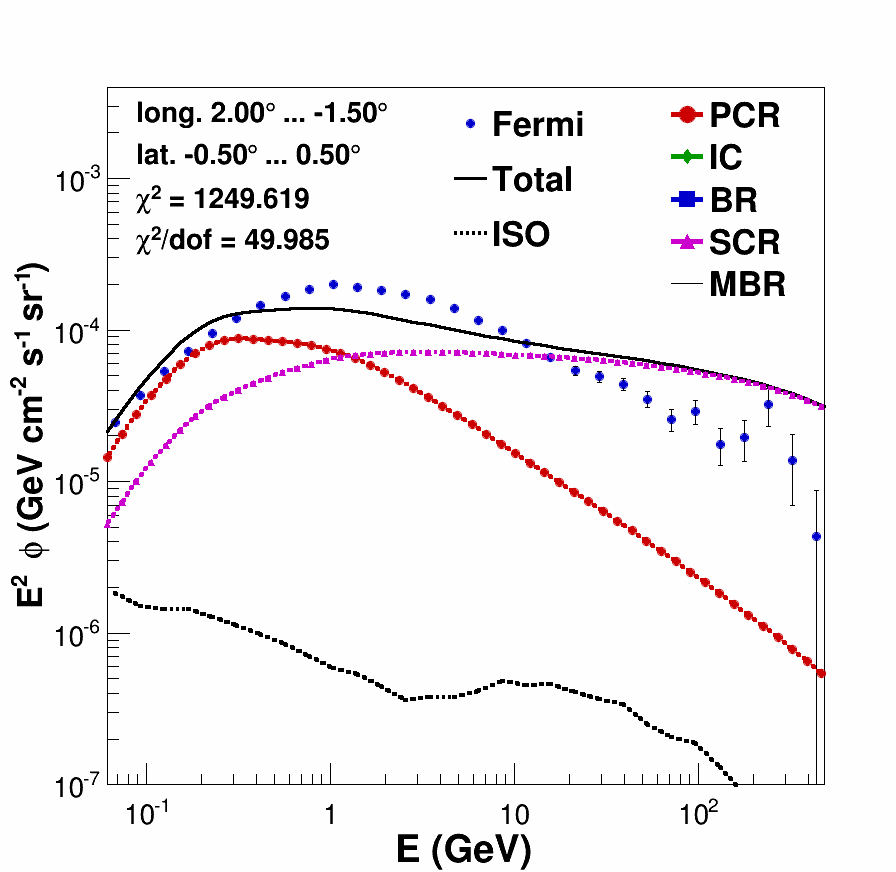
\includegraphics[width=\linewidth]{pic/results/SCRonly_CMZ.png}	  
%  	  \subcaption{}
%	  \label{fig:SCRonly_CMZ}
%  \end{minipage}
%  \hfill
  \begin{minipage}[h]{\textwidth}
	  \centering
	  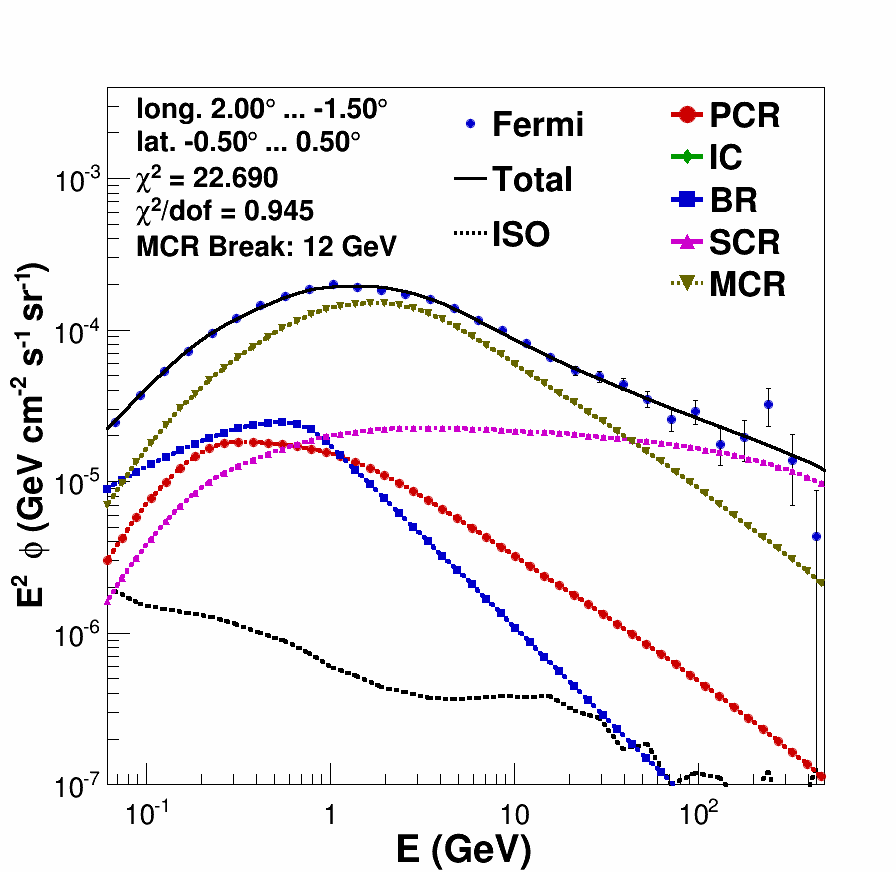
\includegraphics[width=0.5\linewidth]{pic/results/MCRonly_CMZ.png}
%	  \subcaption{}
%  	  \label{fig:MCRonly_CMZ}
  \end{minipage}
  \caption{Fit of the CMZ with PCR, BR, IC, SCR and MCR. The MCR template dominate all the other around 2 GeV, and allow a very low $\chi^2$ value. Compared to Fig. \ref{fig:SCRonly_CMZ_spec}, the SCR component does not overshoot the high energies.}
  \label{fig:MCR_vs_SCRonly_CMZ}
\end{figure}

Fig. \ref{fig:MCR_vs_SCRonly_CMZ} shows the central molecular zone (CMZ) fitted with and without the MCR component. The gas density is very high in this region, hence it is the first region where we would expect the MCR emission to be present. 
Indeed the fit chooses this configuration, with the MCR template dominating all the others and directly improving the fit. The energies around 2 GeV had a clear excess that the four components of the SCR fit could not account for. The MCR template peaking in this region, it comes in very handy and fill this gap, leaving the SCR template taking care of the high energies and the background components for the lower energies.

\todo{Why isn't there IC? -> Wait to see if we change the models}





\newpage
\section{Introducing SCR and DM}
%	-Introduction of SCR + DM
%		-chi2
%		-spatial shapes	
%		-Weniger plots
%		-Specklings
%
%\begin{figure}[h]
%  \centering
%  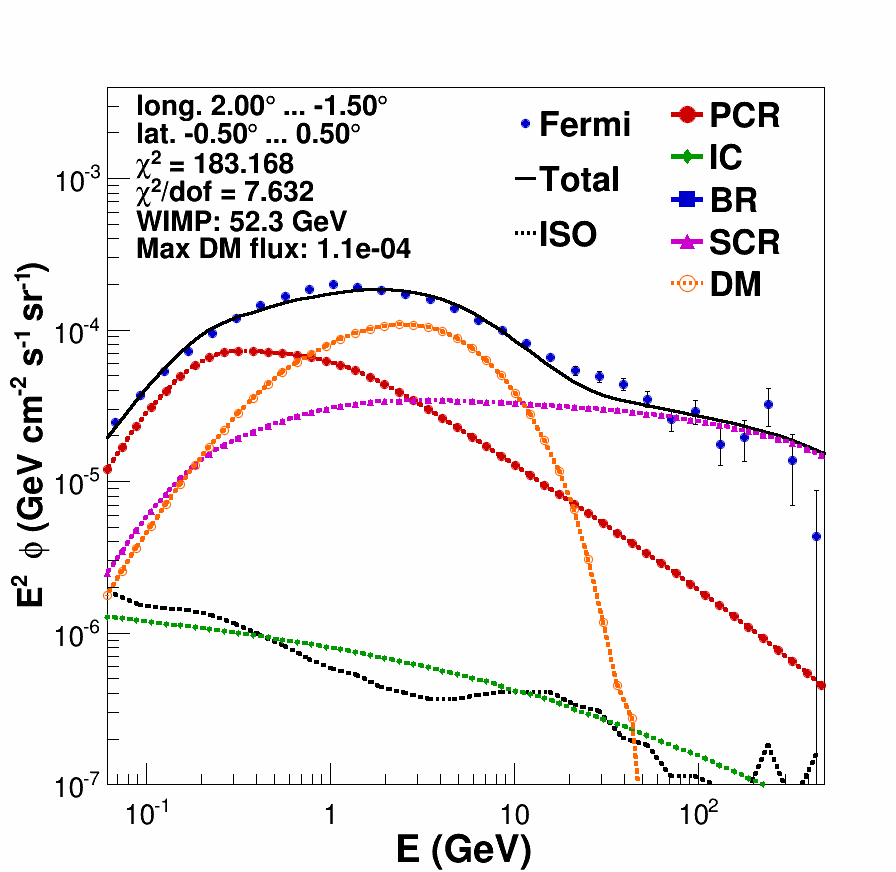
\includegraphics[width=.5\linewidth]{pic/results/DMonly_CMZ.png}
%  \caption{spectrum of best mass DM fitted in CMZ. Also pictures of DM distribution compared to gas map.}
%  \label{fig:DMonly_CMZ}
%\end{figure}

%\begin{figure}[h]
%  \centering
%  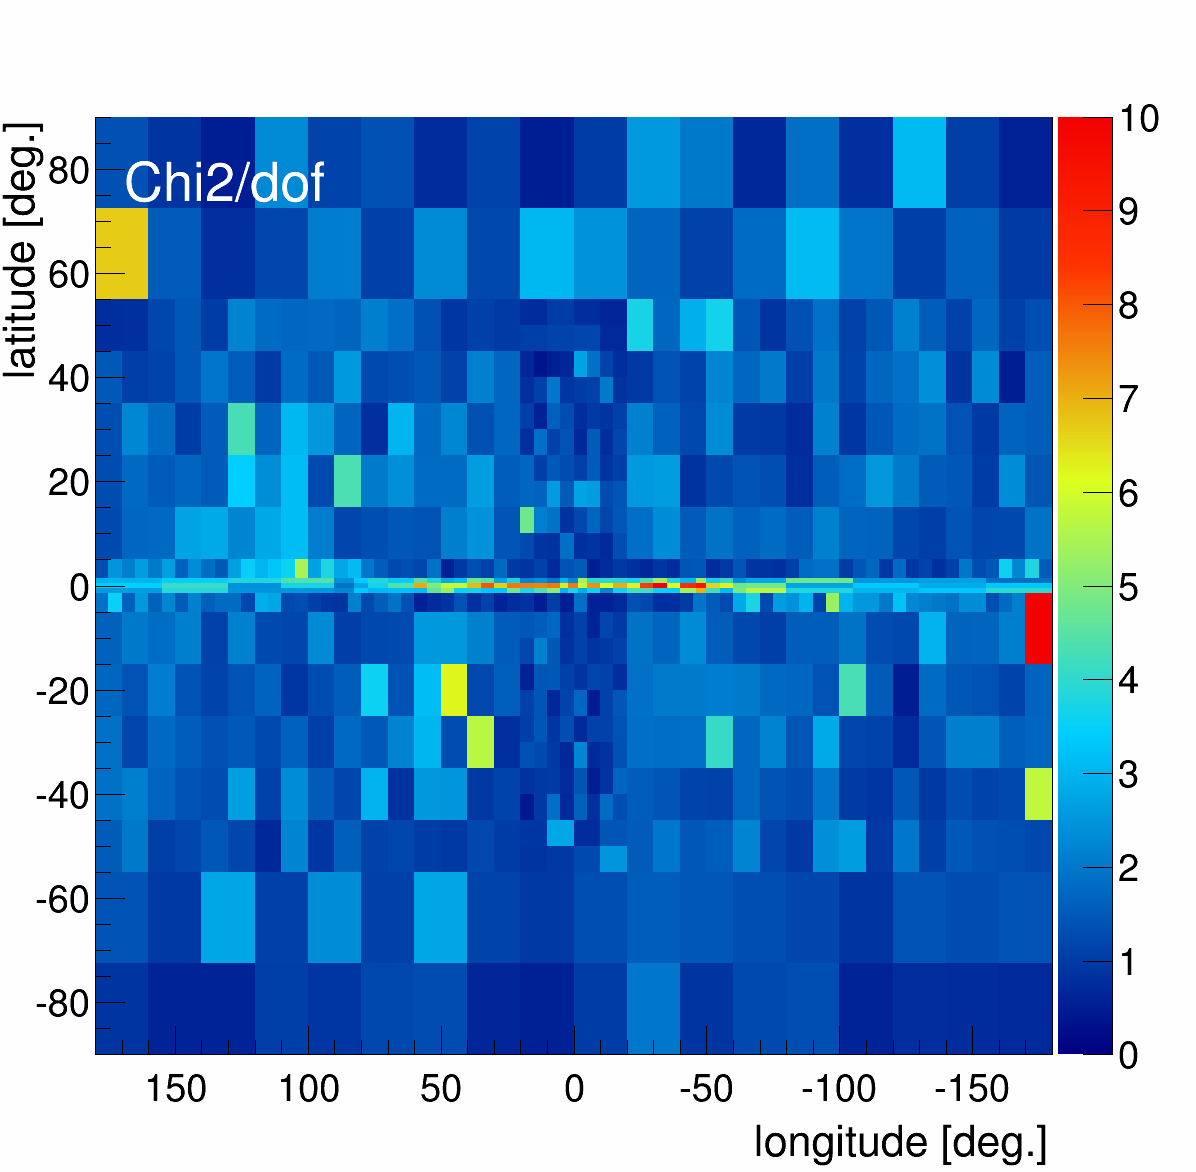
\includegraphics[width=.5\linewidth]{pic/results/DMonly_chi2Distribution.png}
%  \caption{DM fit chi2 distribution}
%  \label{fig:DMonly_chi2Distribution}
%\end{figure}
%
%\begin{figure}[h]
%  \centering
%  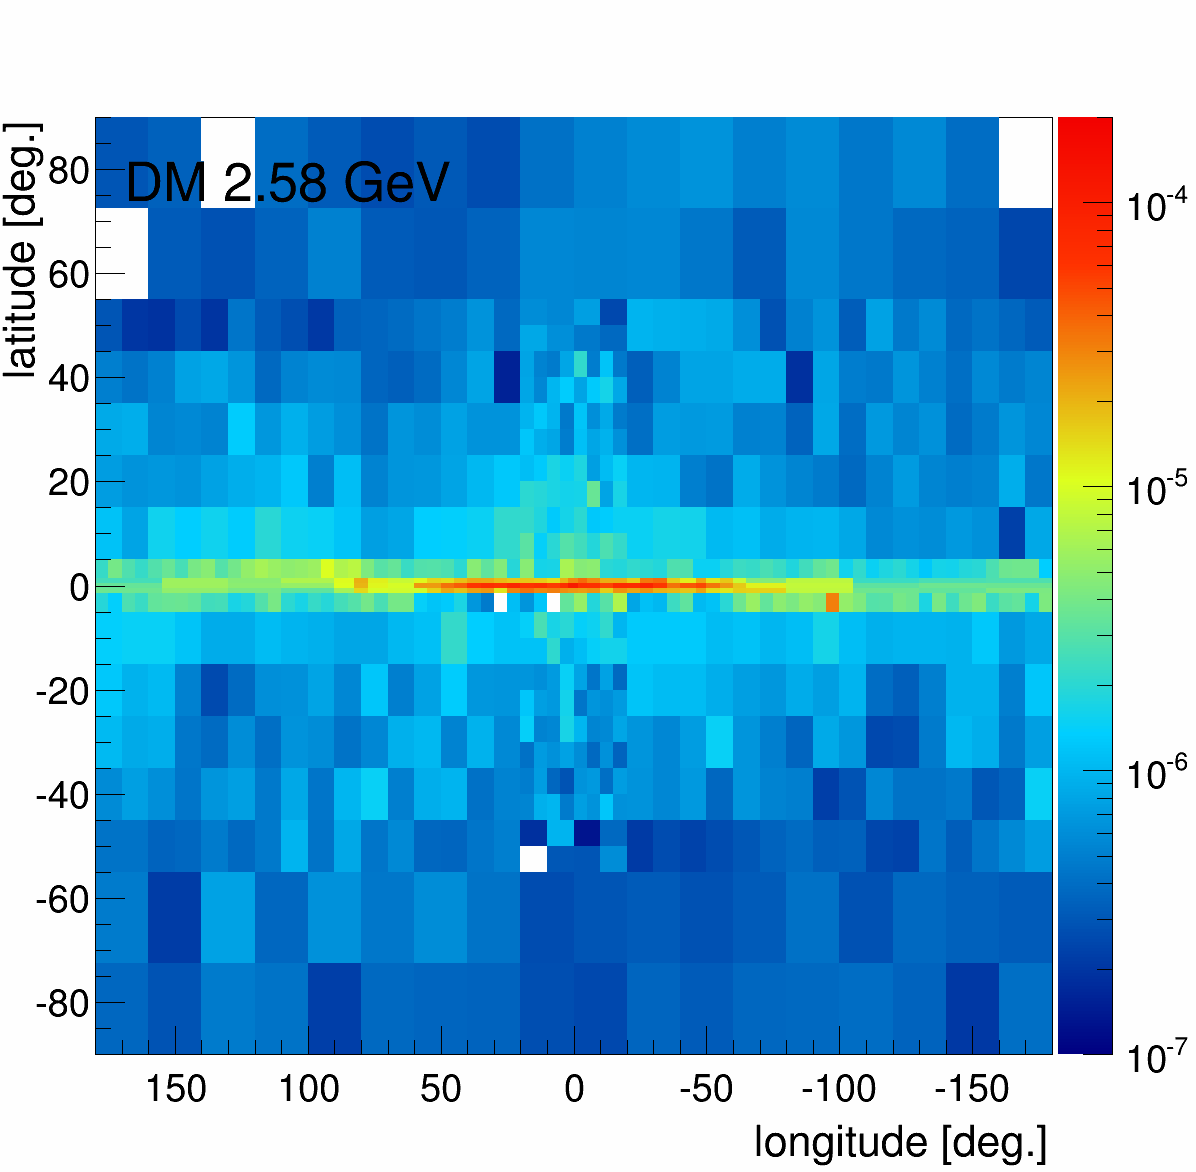
\includegraphics[width=.5\linewidth]{pic/results/DMonly_DM_fluxE12_skymap.png}
%  \caption{DM distribution compared to gas map.}
%  \label{fig:DMonly_skymap_DM}
%\end{figure}
%

Fitting the DM template instead of MCR requires a little more preparation. The first step is to determine which mass for the WIMP particles would produce the best spectrum for our fit. Fig. \ref{fig:DMonly_CMZ} shows the best fit for the CMZ region, with the WIMP mass as a free parameter. This region was chosen to determine the mass because the excess is supposed to dominate the emission. Once the optimum mass for this direction is found, it is fixed and the fit is repeated in the entire sky.
The fit chooses a mass of 52.3 GeV, peaking around a few GeV, as expected in from the excess position.
Once the mass is determined and applied to the entire sky, the fit gives the following results. The $\chi^2$ distribution (Fig. \ref{fig:DMonly_chi2Distribution} is comparable to the MCR fit (Fig. \ref{MCRonly_chi2Distribution}) for the major part but is significantly worst in the disk. This effect would tend to indicate that a DM spectrum is less appropriate to describe the excess, even if nothing can be concluded yet.

Figure \ref{fig:DMonly_CMZ} shows the fit of the CMZ using the DM component as the excess component. A first comparison with the MCR fit points to differences in the higher part of the spectrum. DM is way softer above 10 GeV and this change induces all the differences. This aspect will be discussed later \todo{ref chapter}.



(((As seen on Fig. \ref{fig:DMonly_skymap_DM}, the DM distribution of the fit traces closely the distribution of molecular gas distribution (as traced by CO).)))


\begin{figure}[H]
  \centering
  \begin{minipage}[h]{0.45\textwidth}
  	\centering
	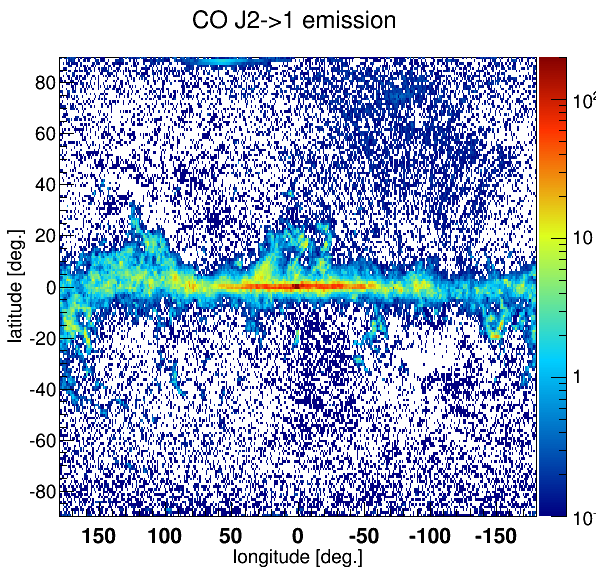
\includegraphics[width=1.\linewidth]{pic/results/COmap.png}
  	\subcaption{CO}
  	\label{fig:CO_skymap}
  \end{minipage}
  \hfill
  \begin{minipage}[h]{0.45\textwidth}
  	\centering
	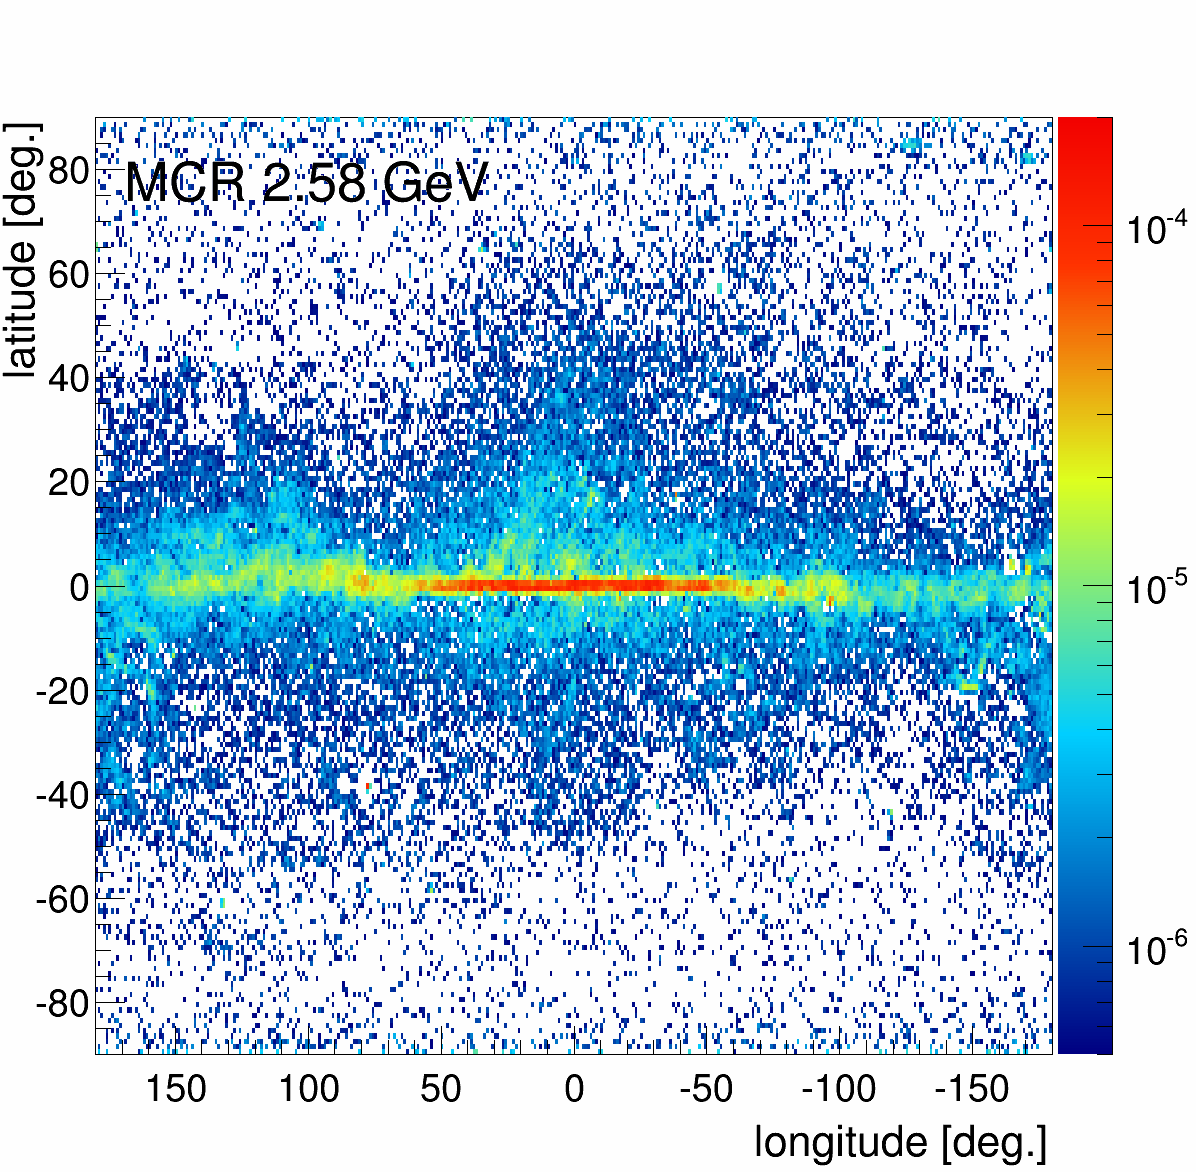
\includegraphics[width=1.\linewidth]{pic/results/MCRonly_fine_MCR_distribution_E12.png}
  	\subcaption{MCR}
  	\label{fig:MCRonly_skymap_MCR}
  \end{minipage}
  \hfill
  \begin{minipage}[h]{0.45\textwidth}
  	\centering
	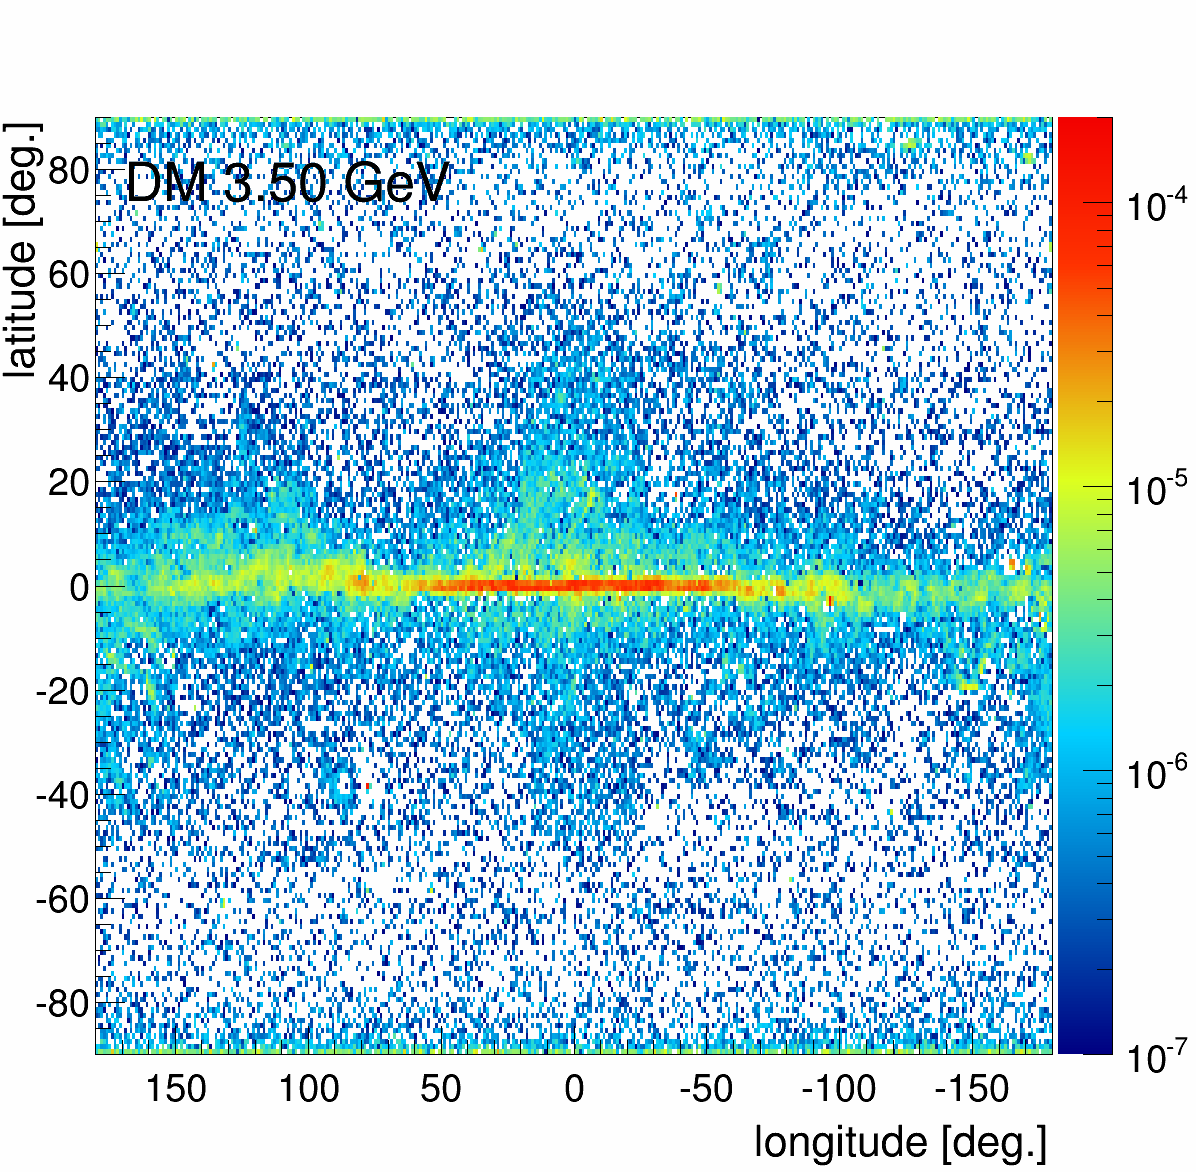
\includegraphics[width=1\linewidth]{pic/results/DMonly_fine_DM_distribution_E13.png}
 	\subcaption{DM}
  	\label{fig:DMonly_skymap_DM}
  \end{minipage}
  \hfill
  \begin{minipage}[h]{0.45\textwidth}
  	\centering
	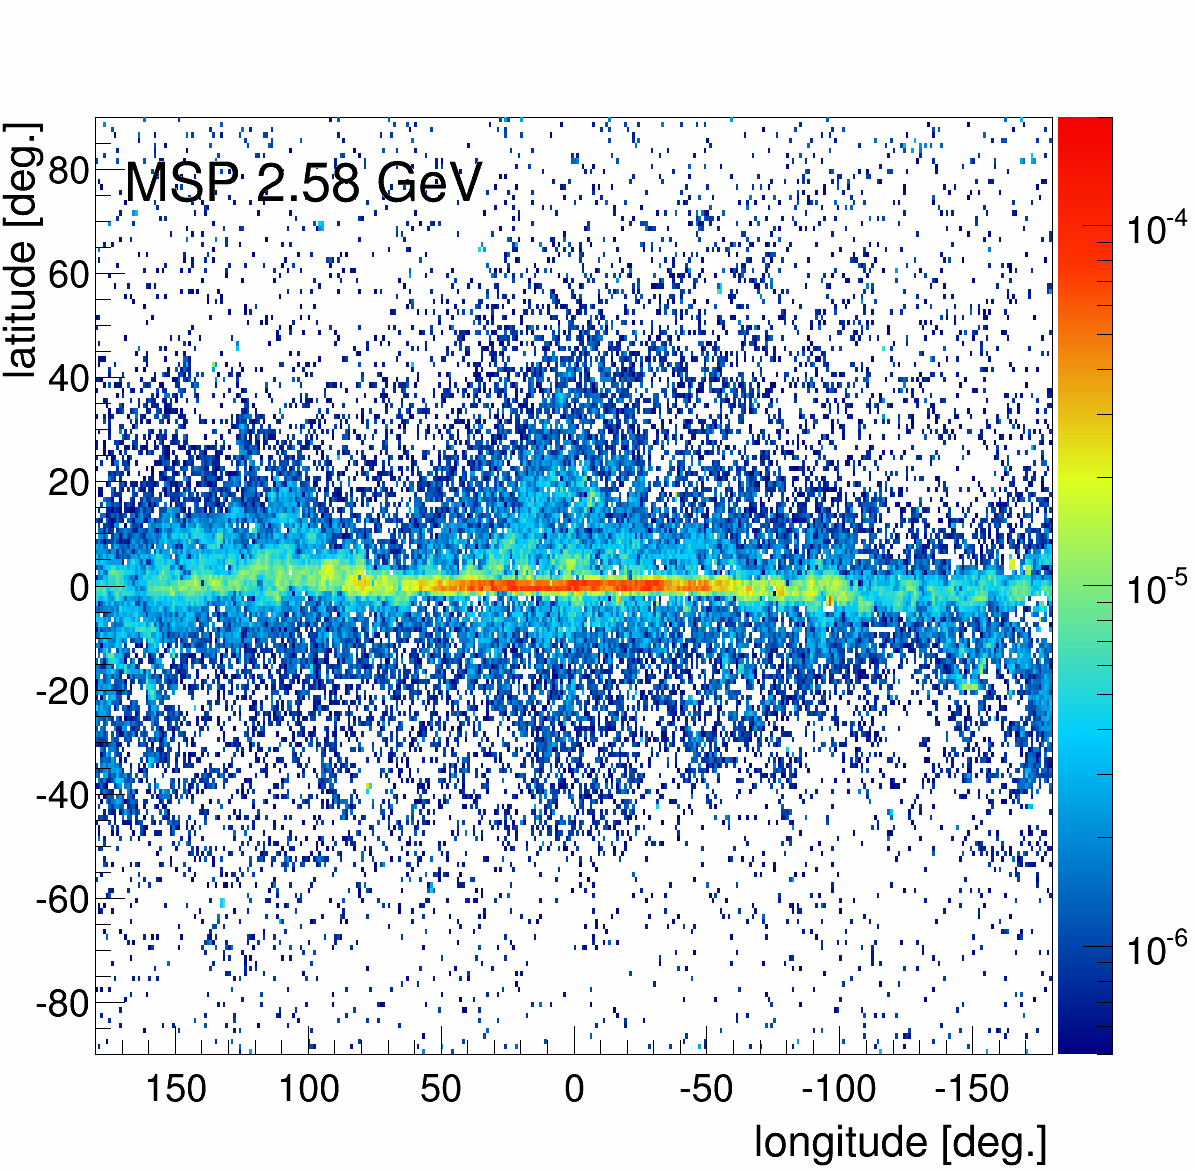
\includegraphics[width=1\linewidth]{pic/results/MSPonly_fine_MSP_distribution_E12.png}
  	\subcaption{MSP}
  	\label{fig:MSPonly_skymap_MSP}
  \end{minipage}
  \caption{Spatial distribution of the flux for CO (a), MCR (b), DM (c) and MSP (d). The same structures appear in all four maps, with the disk clearly delimited between -90 and 90 degrees in longitude and a widening around the GC and 120 degrees in longitude. The distribution of molecular clouds as traced by CO can be found in the excess component distribution, whatever hypothesis is used. This is expected only for the MCR hypothesis, but not for DM or MSP.}
  \label{fig:Excess_comp_flux_comparison}
\end{figure}


\newpage
\section{Introducing SCR and MSP}
%	-Introduction of SCR + MSP:
%		-chi2
%		-spatial shapes
%		-Weniger plots
%		-Specklings
%
%\begin{figure}[h]
%  \centering
%  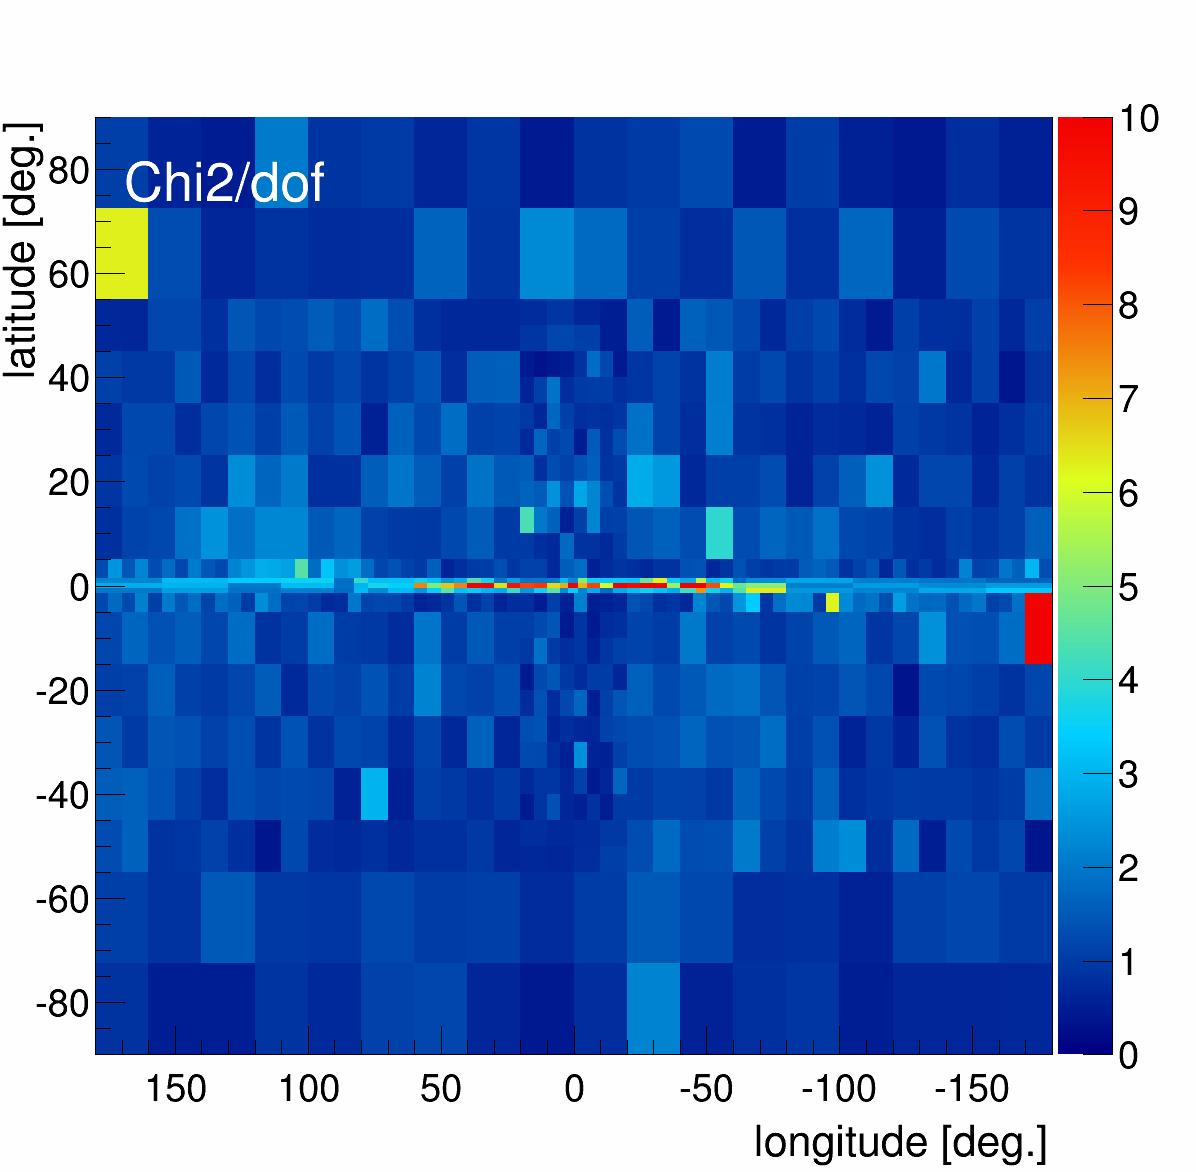
\includegraphics[width=.5\linewidth]{pic/results/MSPonly_chi2Distribution.png}
%  \caption{Chi2 distribution of MSP only fit}
%  \label{fig:MSPonly_chi2Distribution}
%\end{figure}

This section introduces the results of the MSP as the excess component.
The first thing that can be noticed when seeing the $\chi^2$ distribution of the MSP only fit (Fig \ref{fig:MSPonly_chi2Distribution}) is the similitude with the DM only fit (Fig. \ref{fig:DMonly_chi2Distribution}). The fit succeeds pretty well outside the disk, but gets significantly worst for latitudes below two degrees.


Using the MSP spectrum predicted by fermi \cite{Fermi2017} to fit the CMZ region does not give entire satisfaction.
As for DM, the high energy is again too soft and put constraints on other templates.


As shown on Fig. \ref{fig:MSPonly_skymap_MSP}, the distribution of MSP in the sky resembles the distribution of CO, MCR and DM obtained in previous sections. Present everywhere in the disk, with a higher flux in GC and the bubbles.



\todo{add picture of residuals at low energy maybe?}

\newpage
\begin{figure}[H]
  \centering
  \begin{minipage}[h]{0.45\textwidth}
  	\centering
	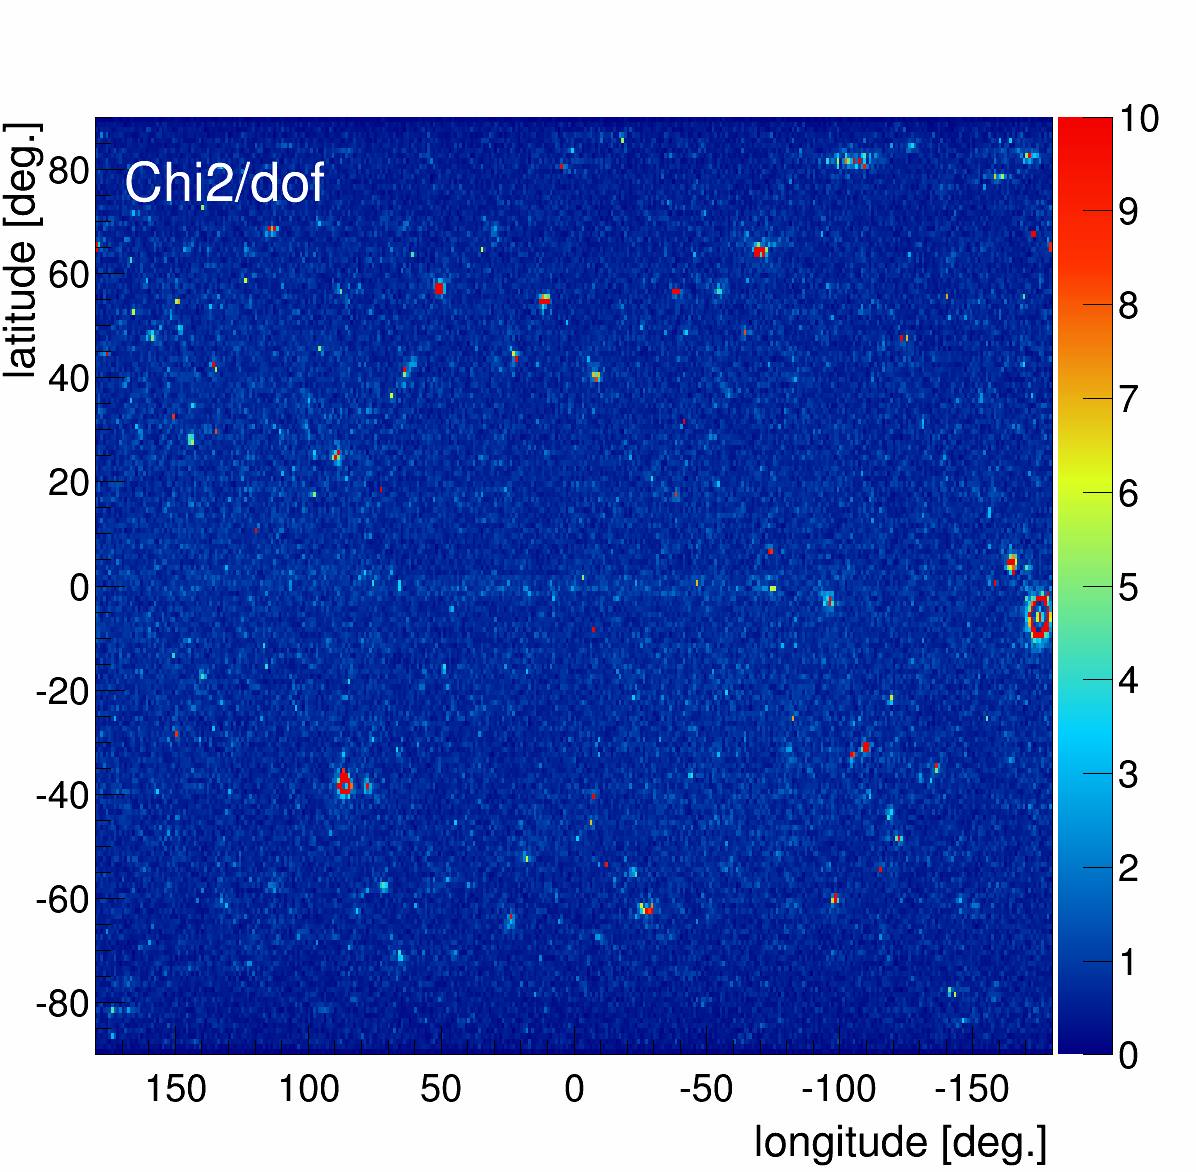
\includegraphics[width=1.\linewidth]{pic/results/MCRonly_fine_chi2_distribution.png}
  	\subcaption{}
  	\label{fig:MCRonly_chi2Distribution}
  \end{minipage}
  \hfill
  \begin{minipage}[h]{0.45\textwidth}
  	\centering
	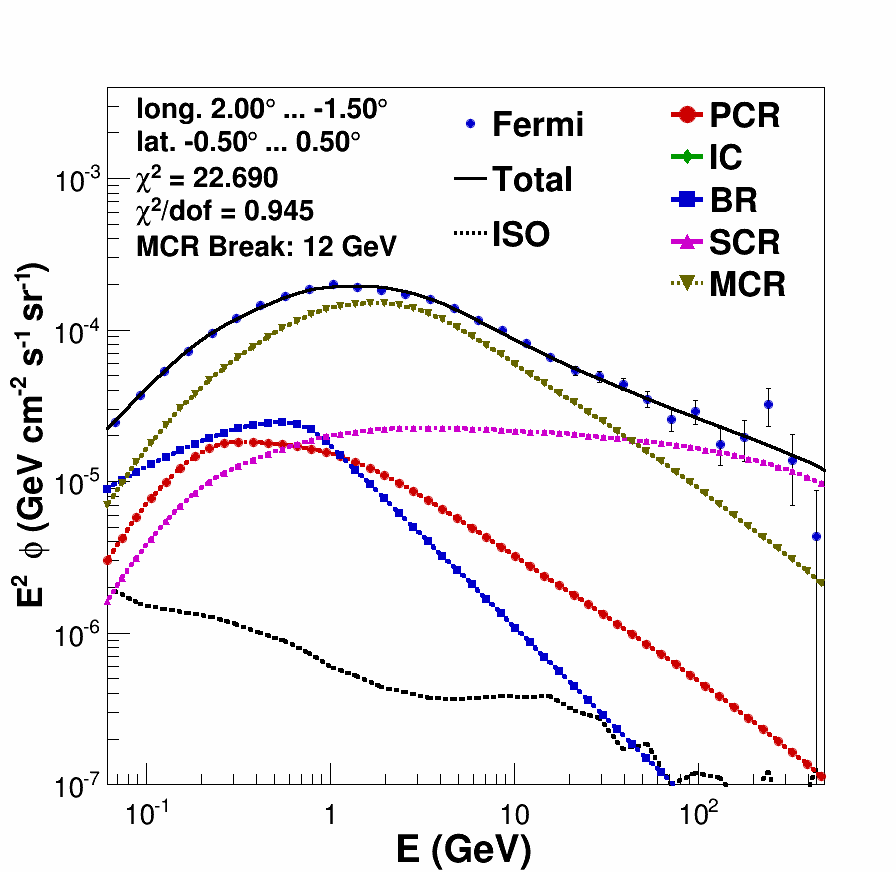
\includegraphics[width=\linewidth]{pic/results/MCRonly_CMZ.png}
	\subcaption{}
  	\label{fig:MCRonly_CMZ}
  \end{minipage}
  \hfill
  \begin{minipage}[h]{0.45\textwidth}
  	\centering
	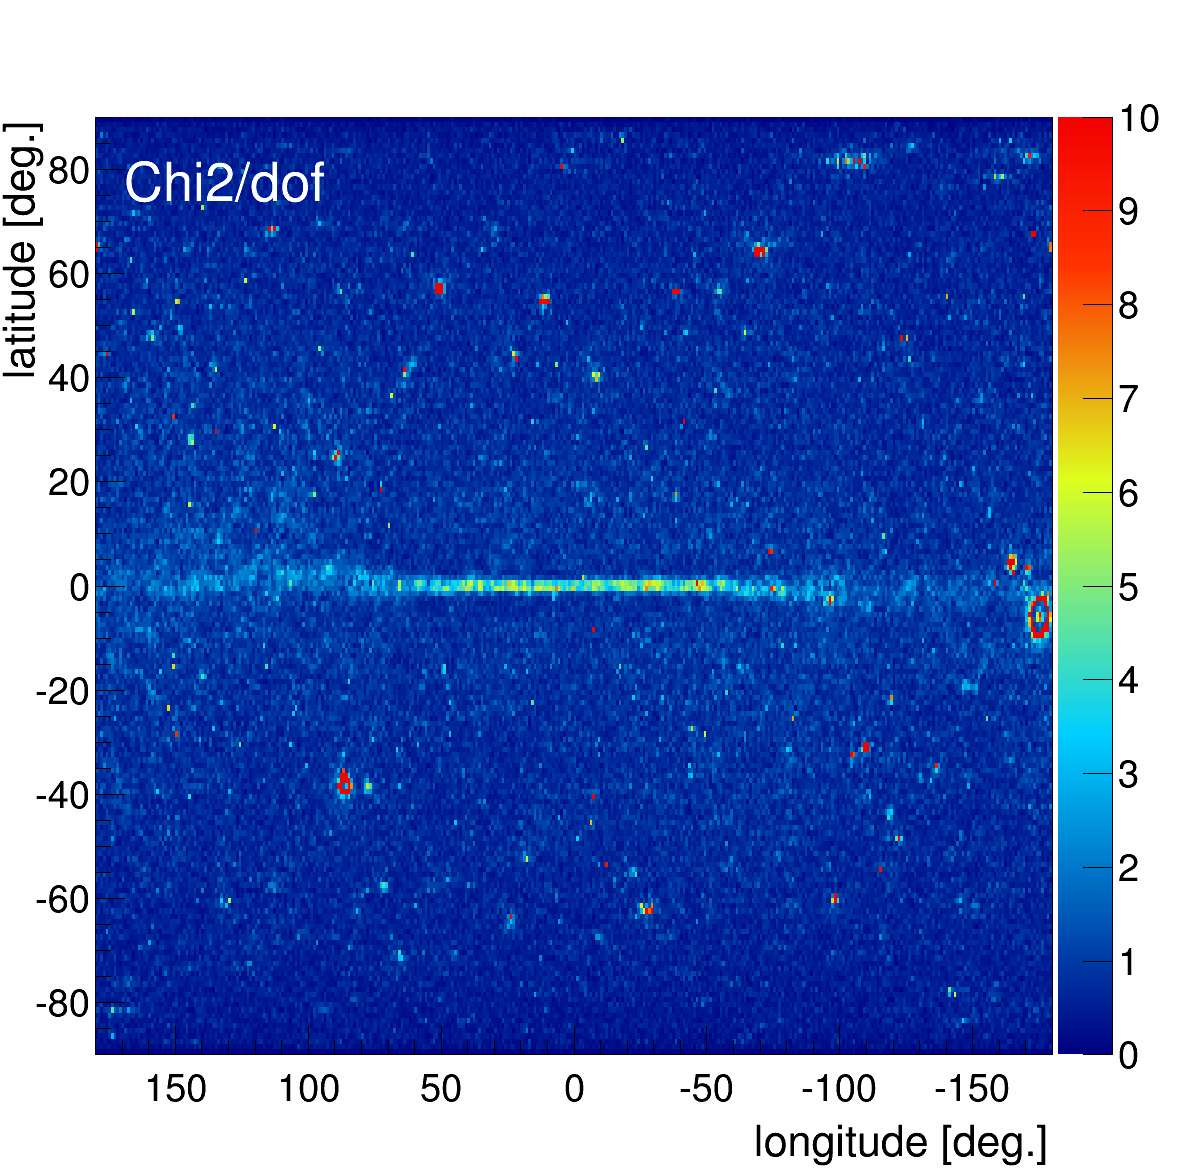
\includegraphics[width=1\linewidth]{pic/results/DMonly_fine_chi2_distribution.png}
  	\subcaption{}
  \label{fig:DMonly_chi2Distribution}
  \end{minipage}
  \hfill
  \begin{minipage}[h]{0.45\textwidth}
  	\centering
	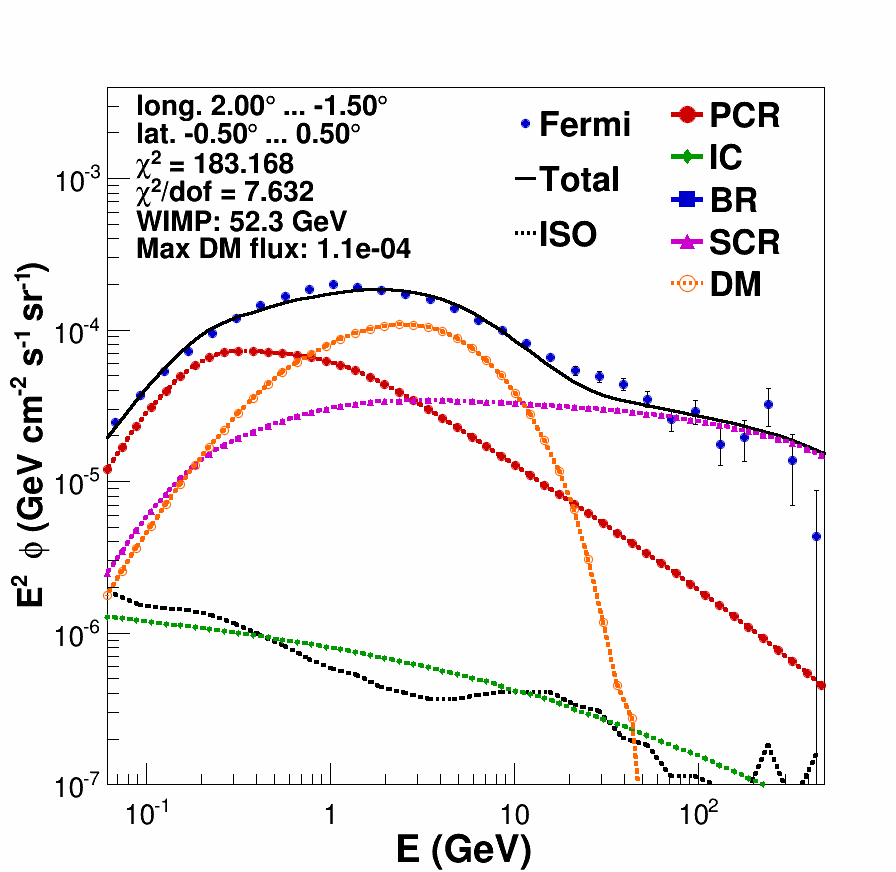
\includegraphics[width=1\linewidth]{pic/results/DMonly_CMZ.png}
  	\subcaption{}
  	\label{fig:DMonly_CMZ}
  \end{minipage}
  \hfill
  \begin{minipage}[h]{0.45\textwidth}
  	\centering
	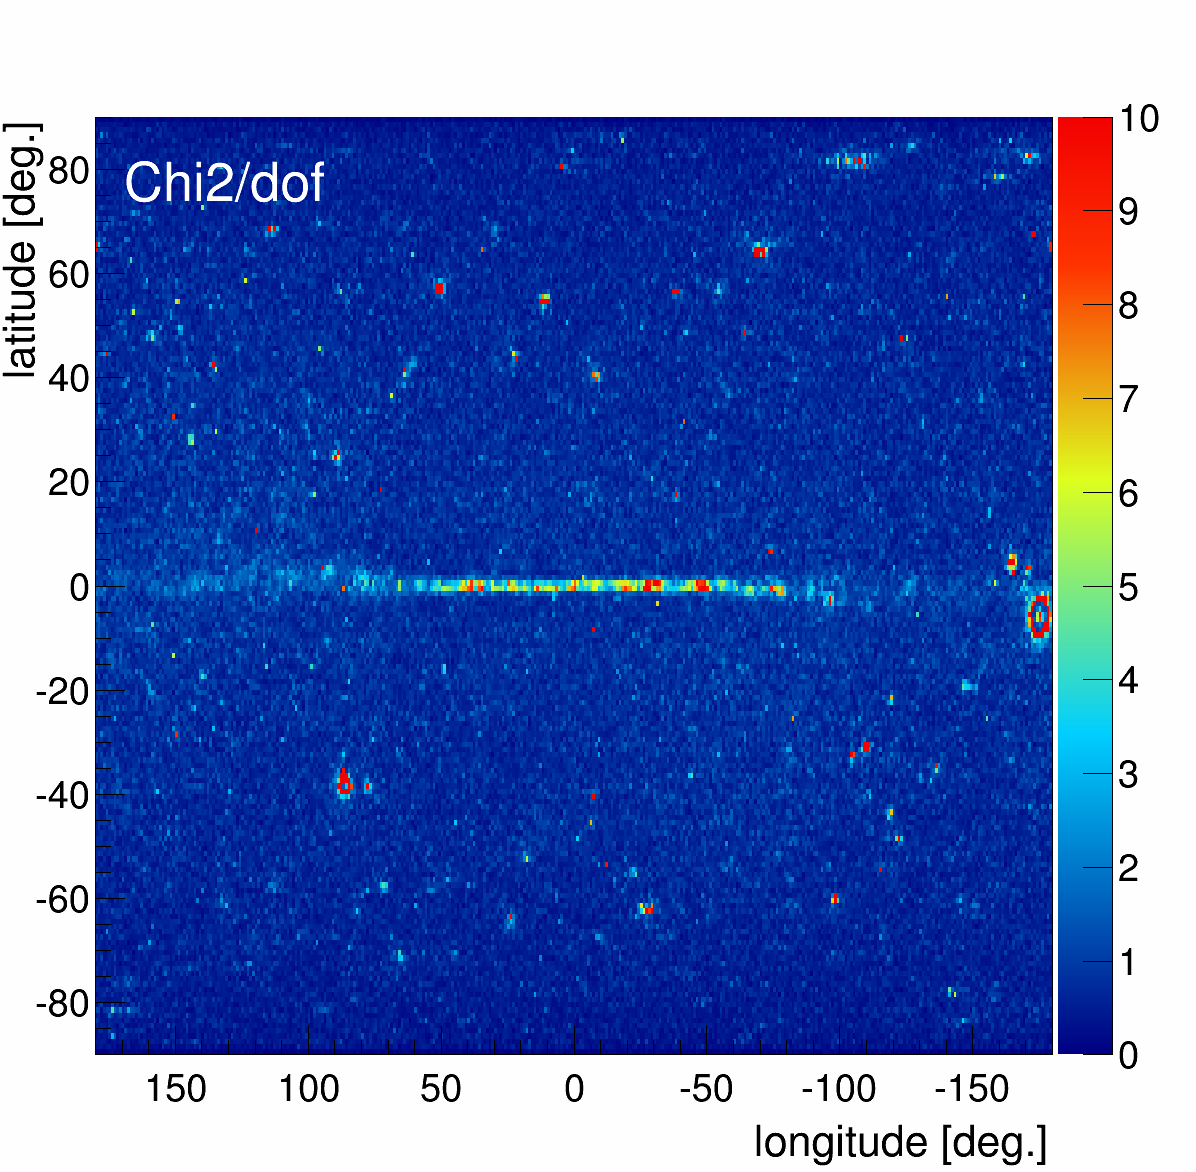
\includegraphics[width=1\linewidth]{./pic/results/MSPonly_fine_chi2_distribution.png}
  	\subcaption{}
  \label{fig:MSPonly_chi2Distribution}
  \end{minipage}
  \hfill
  \begin{minipage}[h]{0.45\textwidth}
  	\centering
	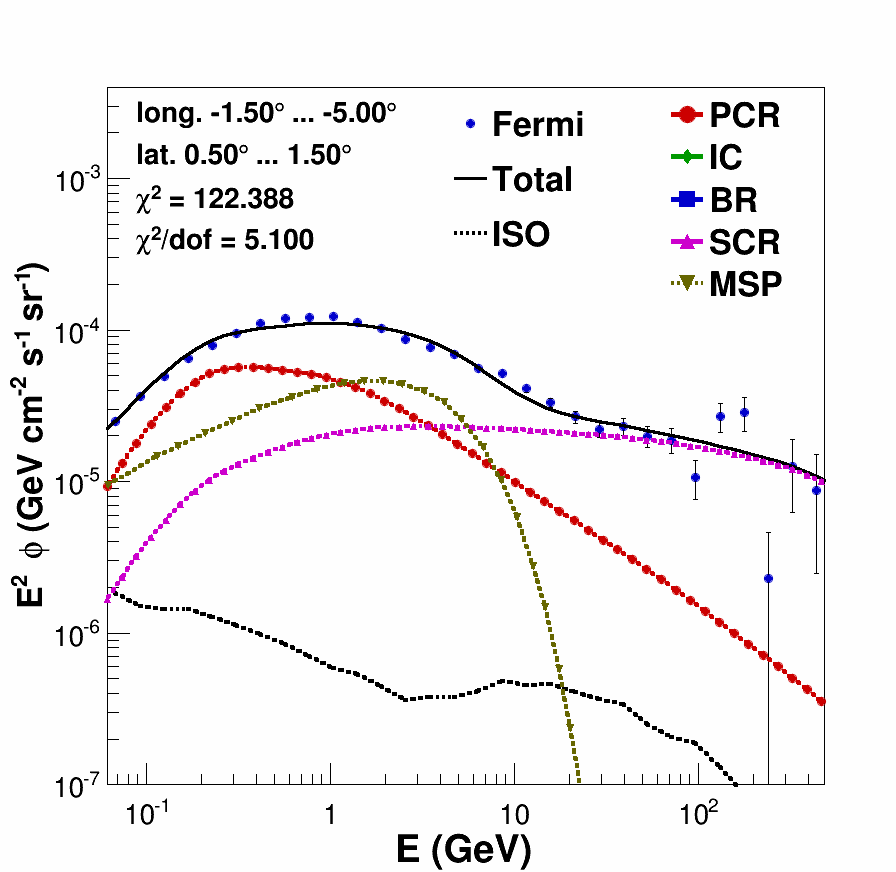
\includegraphics[width=1\linewidth]{pic/results/MSPonly_CMZ.png}
  	\subcaption{}
  	\label{fig:MSP_only_CMZ}
  \end{minipage}
  \caption{Comparison of the $\chi^2$ distributions for the three excess fits (left column) and the CMZ region (right column). MCR (top row), shows a flat $\chi^2$ distribution map, with almost no sign of the disk, and the CMZ is modelled at all energies. DM (middle row) does not fit the disk so well, and the CMZ is not described correctly above 10 GeV. MSP (bottom row) resemble a lot the DM model, with problems in the disk and a poor fit of the CMZ at high energies.}
  \label{fig:Excess_comp_comparison}
\end{figure}





\newpage
\section{Why is MCR better than DM or MSP and a recap of the results so far}
%	-Why is MCR better than DM or MSP
%		-spectral shape of DM
%			-falls off too steep
%		-spectral shape of MSP
%			-Is too soft at low energies
%

Gathering the results of the previous section, a conclusion tends to emerge: the fit clearly prefers the MCR hypothesis over DM and MSP. We will discuss why in this section.

A first step in understanding what is going on can be to compare the $\chi^2$ skymaps. The higher is the $\chi^2$, the worst is the fit. Looking at the background only fit (with PCR, IC and BR only), the disk and the bubbles clearly define a bad $\chi^2$ zone (as seen on Fig. \ref{fig:BKGonly_chi2Distribution}). The high energies are not described at all, with a fitted flux too low (see Fig. \ref{fig:BKGonly_bubble_spec}). It indicates a lack of high energy components that could be able to bring a high energy contribution. This problem is solved by introducing the SCR component and does not play a major role in identifying the excess.

%This template is obtained from a proton injection spectrum with a spectral index of 2.1 (instead of 2.85 for PCR). This harder spectrum is representing the proton population that did not yet diffuse in the galaxy, therefore the high energy protons did not had the time to loose their energy. This new template is expected to be present in the disk and the bubbles. In the disk because there is a very high density of point sources, and the 3FGL catalog does not list them all. These sources can produce gamma-rays from their expelled CRs in their near surrounding, thus providing a very hard proton spectrum. It is also expected in the bubbles since they are also composed of relativistic CR ejected from the GC directly outward the disk. These CRs do not propagates, at least less than in the disk, thus keeping a hard spectrum in those regions.

The first results with SCR added to the three background component is a success with clear improvement in the bubbles. They are not visible anymore when looking only at the $\chi^2$ skymap and this is a very good sign. On the other hand, the disk is still not fitted correctly, as can be seen from the large $\chi^2$ band at latitudes below a few degrees. Even if there is an small improvement, the addition of a fifth component can be beneficial.
Now that the high energies are taken care of, the excess shows around a few GeV. There are three different candidates for the job: MCR, DM and MSP. All three correspond to a unique process with clear definitions and expectations.



The first hypothesis to be proposed for this excess was the presence of DM in the GC. As explained before, the DM halo is expected to be spherical around the GC following a NFW profile, since it does not interact with matter. And since the gamma-ray production from DM is directly proportional to the DM density, the DM component is expected to be spherical around the GC as well. There is no reasons for it to be correlated with the spatial shape of the Milky Way. But looking at the results (Fig. \ref{fig:DMonly_skymap_DM}), the fit does not meet these theoretical expectations for DM distribution. The DM flux follows the bar shape of the galaxy, with a high flux below two degrees in latitude and ninety degrees in longitude. Then, some distinct objects can be identified in the disk, around -90 and 90 degrees in longitudes. \todo{remember their names}.
The MSP fit, also expected to have a spherical distribution of gamma-rays from millisecond pulsars, gives similar results. The flux seems to be needed by the fit to describe the disk and regions with molecular clouds as traced by CO in general.
In both cases, the $\chi^2$ maps show an improvement of the model, but the morphology of the new components tends to disagree with the theory.


%Even if the $\chi^2$ in the disk is improved everywhere, it is not sufficient to say that the observed excess is due to DM. First because there are still some regions near the GC where it stays high, and because the distribution of DM predicted by the fit is not spherical at all. On the contrary, it seems to follow the disk and gas distribution when comparing the DM and CO maps \todo{add figure}.


The addition of MCR leads once again to the same kind of results, but this time, the spatial distribution is expected to follow the MCs. The $\chi^2$ map is a little better than for the other two with the disappearance of the remaining bad fits in the disk. A $\chi^2$ around one is obtain on the entire sky. 
The fact that this distribution tends to be the same for all three additional component could be expected, since their energy spectra are similar, and the excess they are supposed to describe has a fixed distribution. But the interesting point is that no spherical distribution is ever observed, nor needed, to fill the 2 GeV excess. 
The only differences in the models for the three excess component is the way theory and results matches. For DM and MSP, the results do not correspond to the predictions, when, on the contrary, MCR theory predicts the obtained morphology.

This quick comparison of the excess component distributions and the $\chi^2$ maps gives a good overview of the results. But even if a preference for MCR can start to emerge, further investigation is preferable before being able to conclude.


\subsection{Comparison of the excess spectral shape}

The only difference between the three excess components that the fit cares about is their spectral shape. It is explained in the chapter \ref{ch:method} that all three templates peak around 2 GeV, but the slopes at low or high energies are different. For energies inferior to 2 GeV, MCR and DM have a similar shape, when MSP is much softer. For energies above 2 GeV, it is the MSP and DM spectrum that look alike, with a very soft spectrum, when MCR is harder.

These differences are the only reasons the fits does not give exactly the same results three times.
Indeed, the low energy spectrum of Fermi data in the disk is relatively hard and does not vary significantly along longitude \todo{add fig}. This plays a major role in differentiating MSP on one side, and MCR and DM on the other. The MSP spectrum being softer than Fermi at low energies, the lowest Fermi data point is limiting the MSP contribution. And the relative contribution of the MSP at 2 GeV can not exceed a certain value due to this soft energy spectrum. On the other hand, the MCR and DM spectra fall down with the same index than the data. Thus, the limit on MCR and DM relative contribution is not as limited by low energies as it is for MSP.
This spectral particularity keeps MSP low and does not allow it to account completely for the excess in the GC.
\todo{add a picture or two, illustrating this effect. maybe two spectra with horizontal lines}


On the other side of the spectrum, above 2 GeV, it is MCR that behave differently than MSP and DM with a harder spectrum. When DM and MSP are completely insignificant above 50 GeV, MCR still plays a role at least as important as the PCR spectrum since they both have the same spectra at high energies. Above 4 GeV, the Fermi data present an constant spectral index with very little variations in the disk. This makes all the difference to distinguish between MCR and MSP or DM. In fact, the important point here is the energy at which the SCR component cross the excess component. In the CMZ, this turnover happens at 50 GeV for MCR, against only 10 GeV and 6 GeV for DM and MSP respectively. This causes the total flux in the DM and MSP fits to present a dip around 11 GeV with a clear change in spectral index. This does not follow the shape of the data. Because of this, the SCR has to overshoot the very high energies (above 100 GeV), to minimize the size of the dip. The PCR component could be a good help with a constant spectral index at high energies, but its contribution is limited by low energies. Indeed, the PCR spectrum peaks around 200 MeV where the Fermi data are already decreasing rapidly. Overall, the MCR spectrum presents the right shape at high energies, with a constant spectral index hard enough to combine wih the SCR component and closely follow the data.


In total, two major differences in the spectral shape of the three excess components could be enough to predict the most adapted one. The low energy spectral index difference between the MSP and the Fermi data leaves the MSP behind the MCR and DM hypothesis. Furthermore, the harder spectrum of MCR at high energies improve the fit significantly compared to MSP and DM. So the only spectrum that presents the right shape at low and high energies is MCR, making him the best candidates for a good model.


%\subsection{Comparison of the excess spatial distribution}
%
%Fig. \ref{fig:MCRonly_skymaps} shows the spatial distribution of the flux of each component around 2 GeV, as returned by the fit.
%
%The bremsstrahlung component is consistent with the the expectations. Present everywhere, it is strong in the disk, and decrease a little in the bubbles.
%
%\todo{Though the general shape is spherical, the IC component has an unexpected feature in the form of a strong depletion in the disk, like a "sandwich" structure. This is surprising in the sense that this is where the interstellar radiation field (ISRF) and electron density are supposed to be maximal, creating a higher IC flux. A possible explanation could be coming from the dust distribution, screening the starlight component of the ISRF. Thus depriving the ISRF of its main component and leaving only the dust infra red emission and the CMB to interact with the electrons. This could result in a lower IC gamma-ray flux in the disk.}
%
%The SCR component is playing his role, filling the bubbles and the disk, where the high energy portion of the spectra needs a harder spectrum. It traces the sources distribution in the disk and the outflow of high energy protons in the bubbles.
%
%The general shape of PCR looks coherent with he shape of the galaxy, with a strong flux in the bar and the galactic disk in general. When looking closely, one can see the same kind of depletion in the disk than for IC, even if the effect is less remarkable. This finds its cause in the MCR distribution with a very high flux in the disk. The sum of both templates (MCR + PCR) shows no sign of such a feature, which tends to show that some of the PCR photons are absorbed by the MCR template. But the total is coherent, with no unexplainable central gap.
%
%The MCR template also follows the spatial distribution of molecular clouds in our galaxy. It is a good sign since it is supposed to come from those regions.
%It is not spherical at all. That could have happened if the excess component has a DM origin, since it is supposed to be spherically distributed.

%
%\newpage
%\begin{figure}[h]
%  \centering
%  \begin{minipage}[h]{0.45\textwidth}
%  	\centering
%	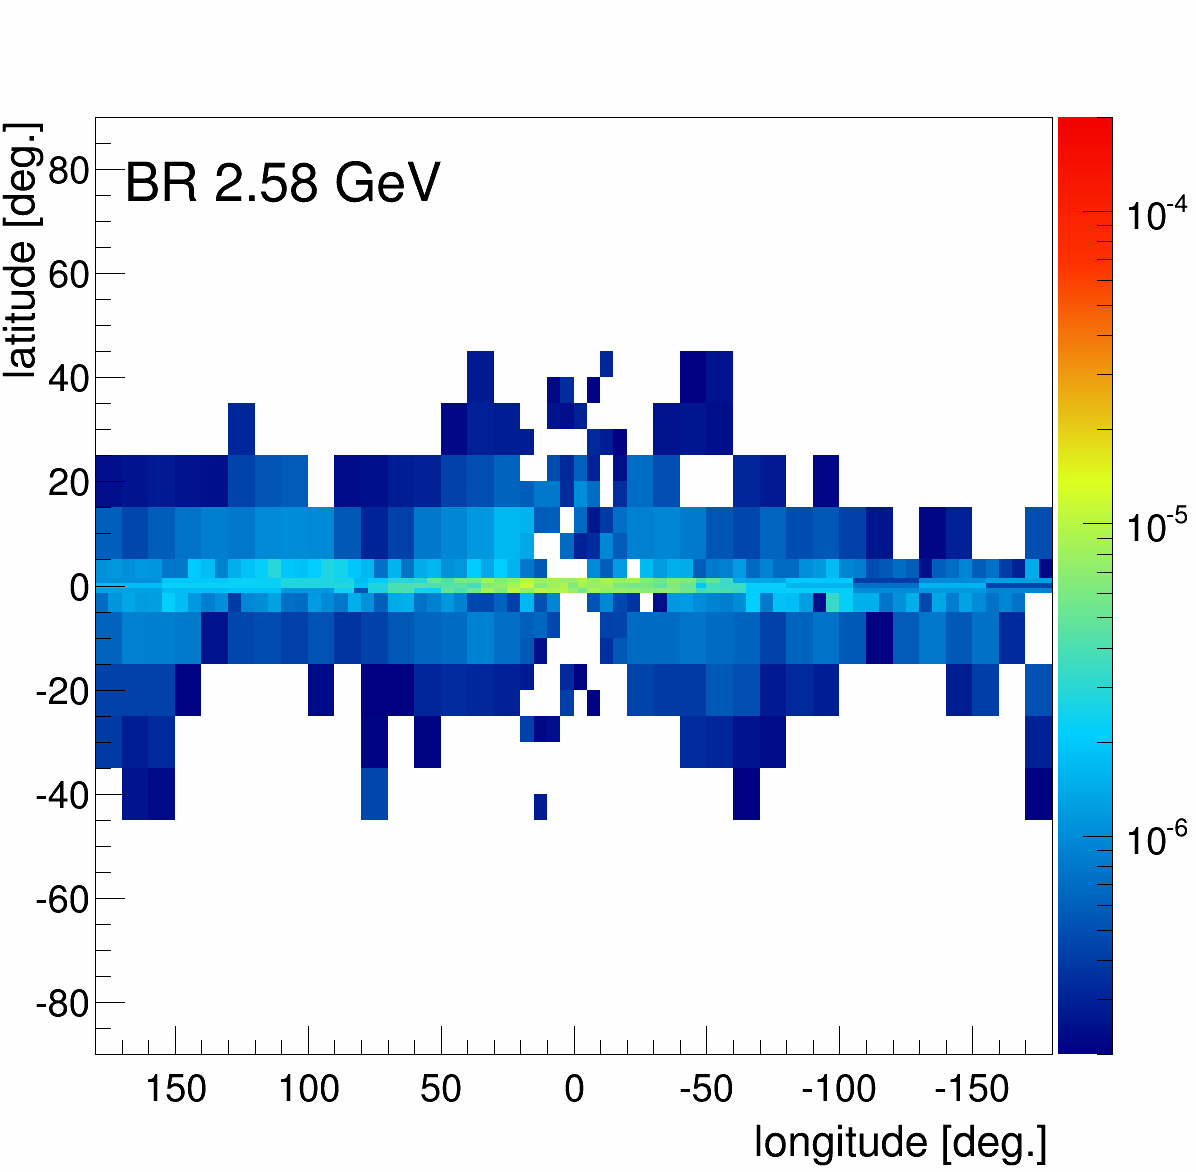
\includegraphics[width=1.\linewidth]{pic/results/MCRonly_BR_fluxE12_skymap.png}
%  	\subcaption{Flux distribution of bremstrahlung (BR)}
%  	\label{fig:MCRonly_skymap_BR}
%  \end{minipage}
%  \hfill
%  \begin{minipage}[h]{0.45\textwidth}
%  	\centering
%	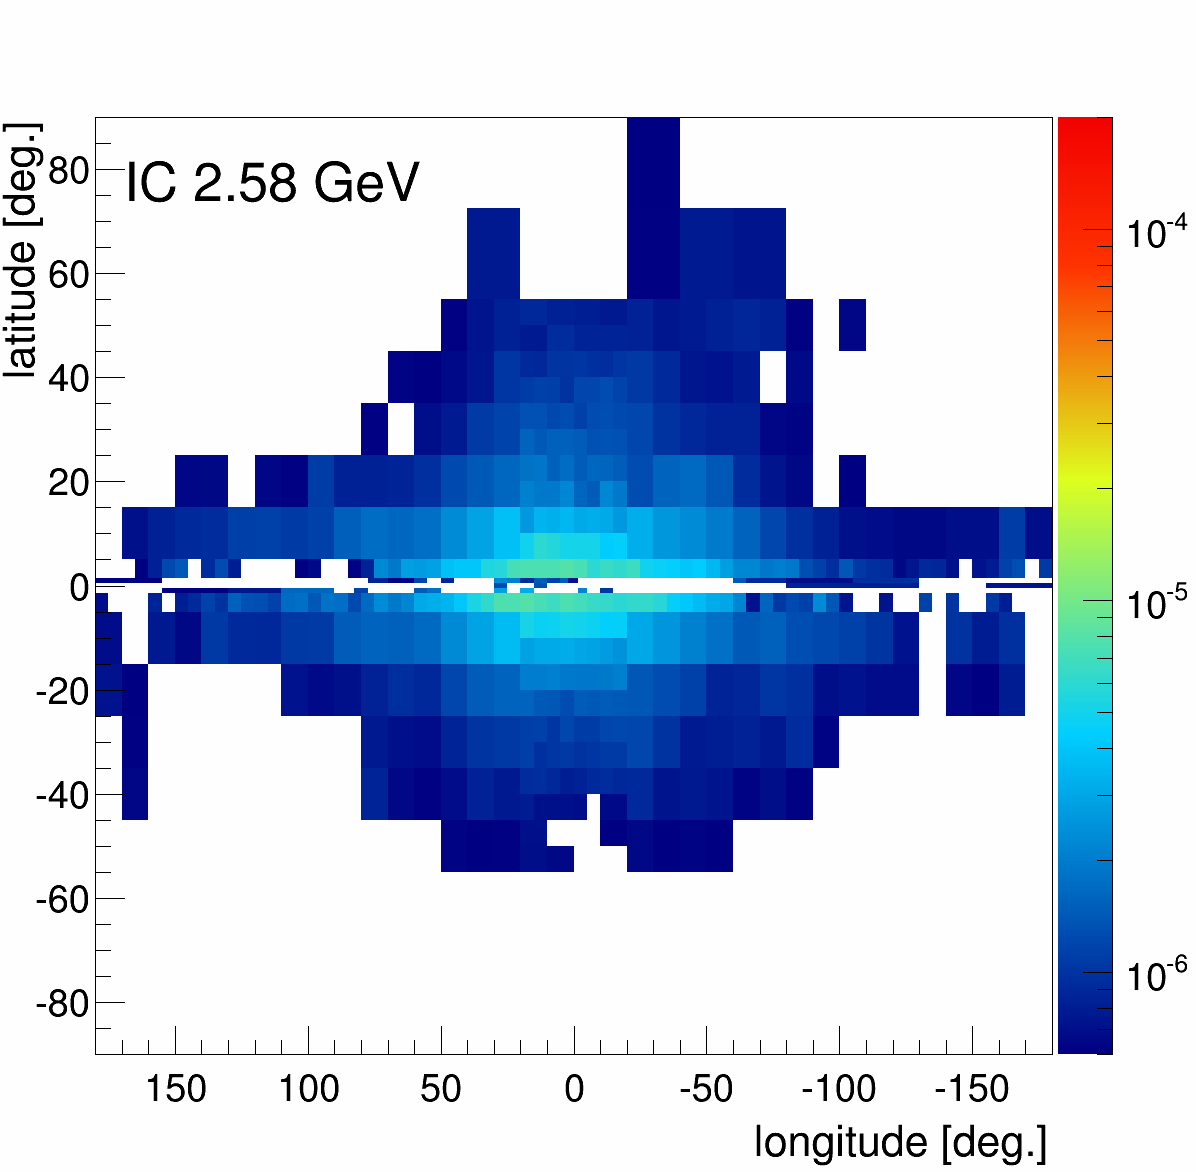
\includegraphics[width=1.\linewidth]{pic/results/MCRonly_IC_fluxE12_skymap.png}
%  	\subcaption{Flux distribution of inverse compton (IC)}
%  	\label{fig:MCRonly_skymap_IC}
%  \end{minipage}
%  \hfill
%  \begin{minipage}[h]{0.45\textwidth}
%  	\centering
%	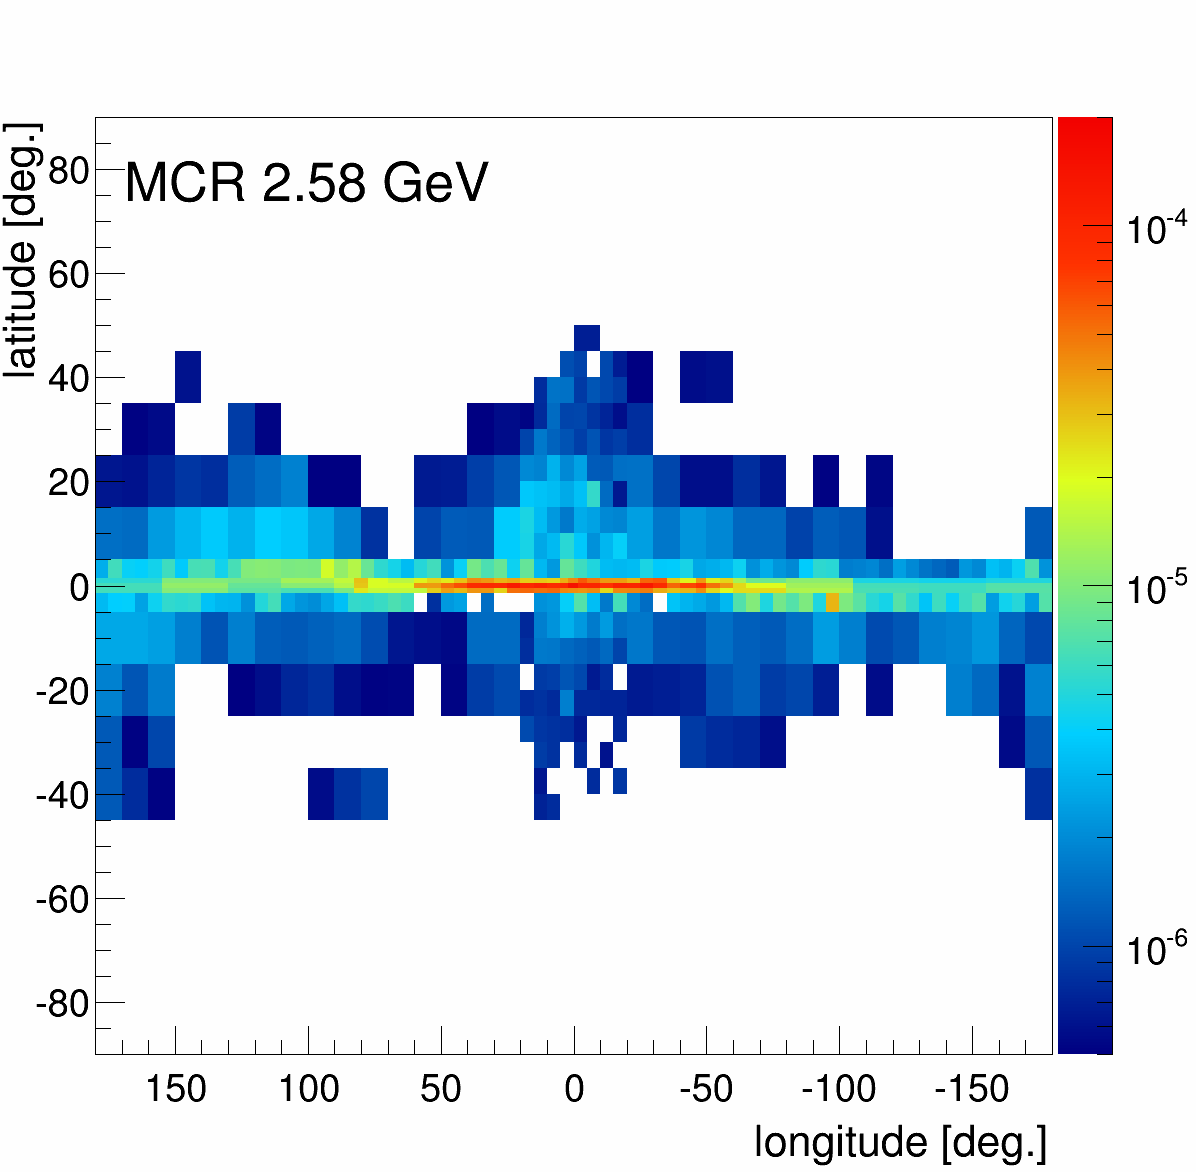
\includegraphics[width=1.\linewidth]{pic/results/MCRonly_MCR_fluxE12_skymap.png}
%  	\subcaption{Flux distribution of MCR}
%  	\label{fig:MCRonly_skymap_MCR}
%  \end{minipage}
%  \hfill
%  \begin{minipage}[h]{0.45\textwidth}
%  	\centering
%	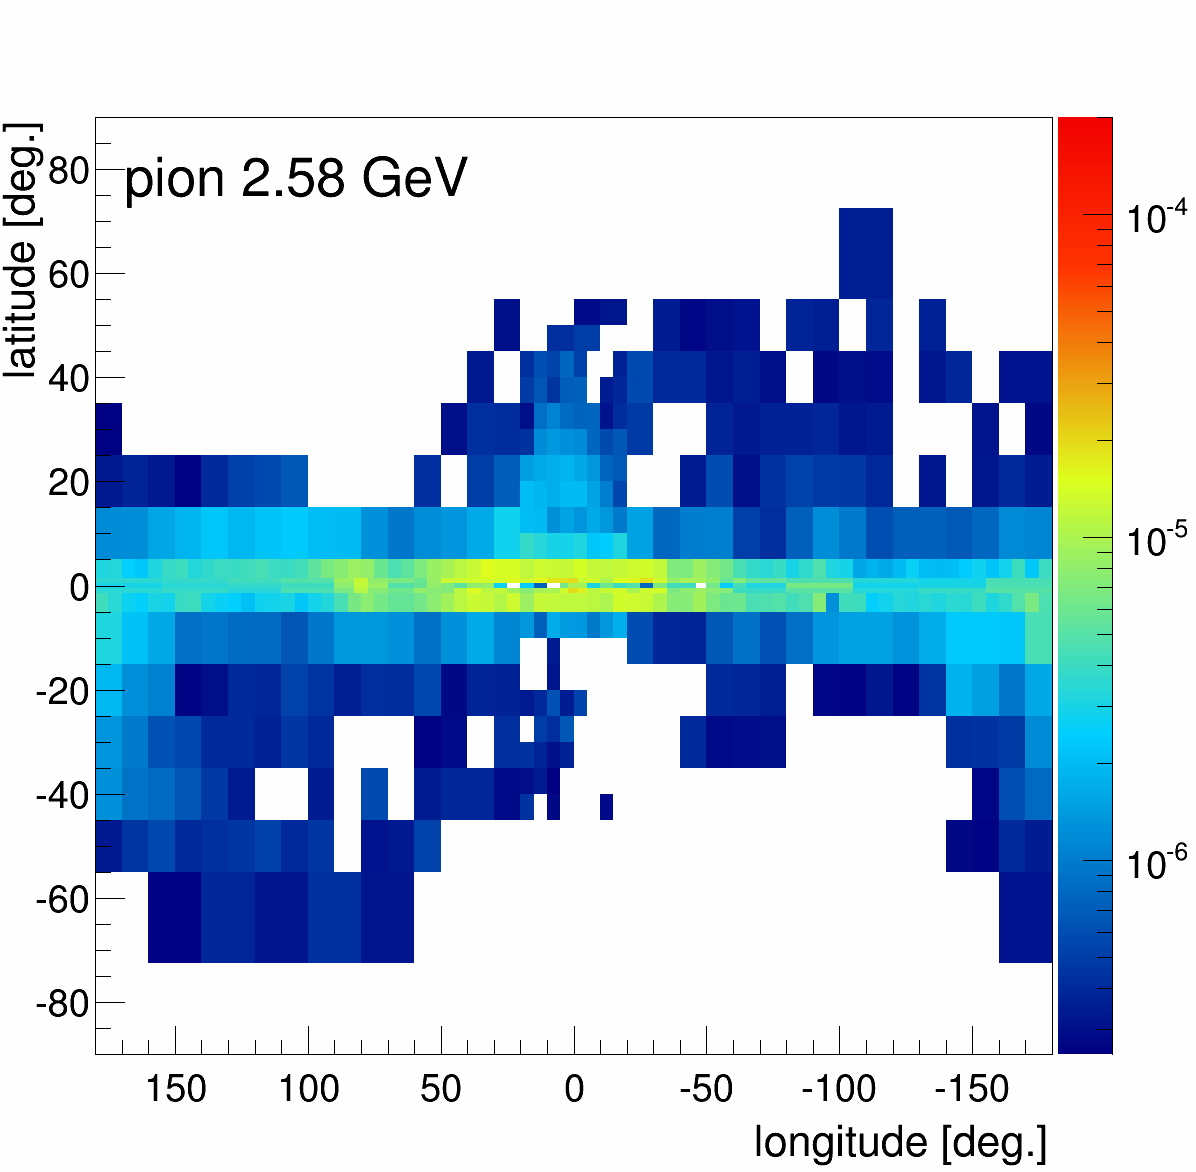
\includegraphics[width=1.\linewidth]{pic/results/MCRonly_PCR_fluxE12_skymap.png}
%  	\subcaption{Flux distribution of PCR}
%  	\label{fig:MCRonly_skymap_PCR}
%  \end{minipage}
%  \hfill
%  \begin{minipage}[h]{0.45\textwidth}
%  	\centering
%	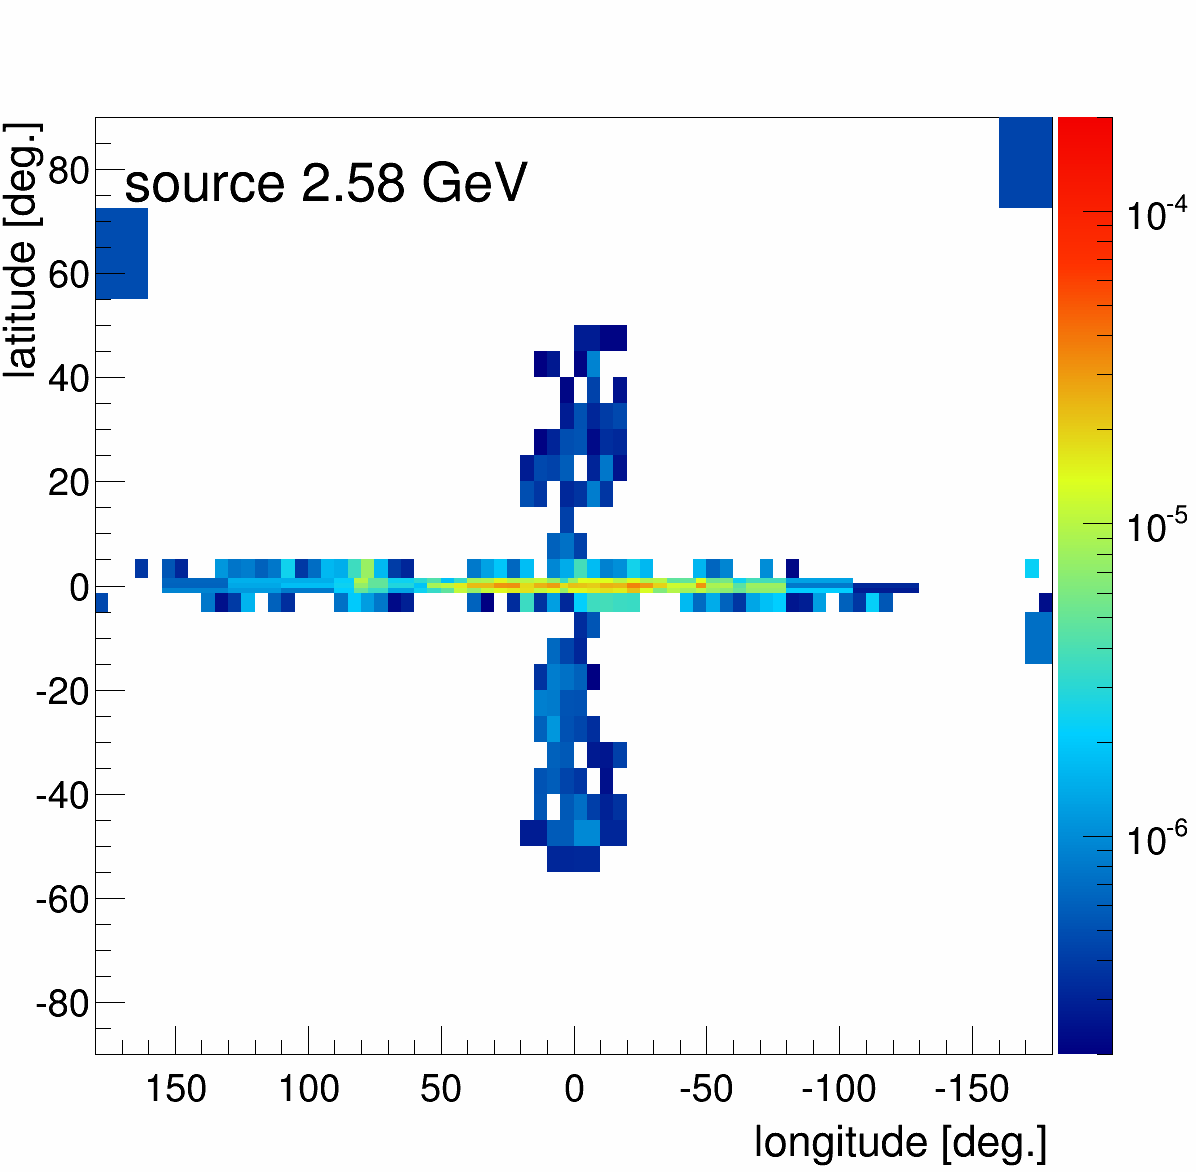
\includegraphics[width=1.\linewidth]{pic/results/MCRonly_SCR_fluxE12_skymap.png}
%  	\subcaption{Flux distribution of SCR}
%  	\label{fig:MCRonly_skymap_SCR}
%  \end{minipage}
%  \hfill
%  \begin{minipage}[h]{0.45\textwidth}
%  	\centering
%	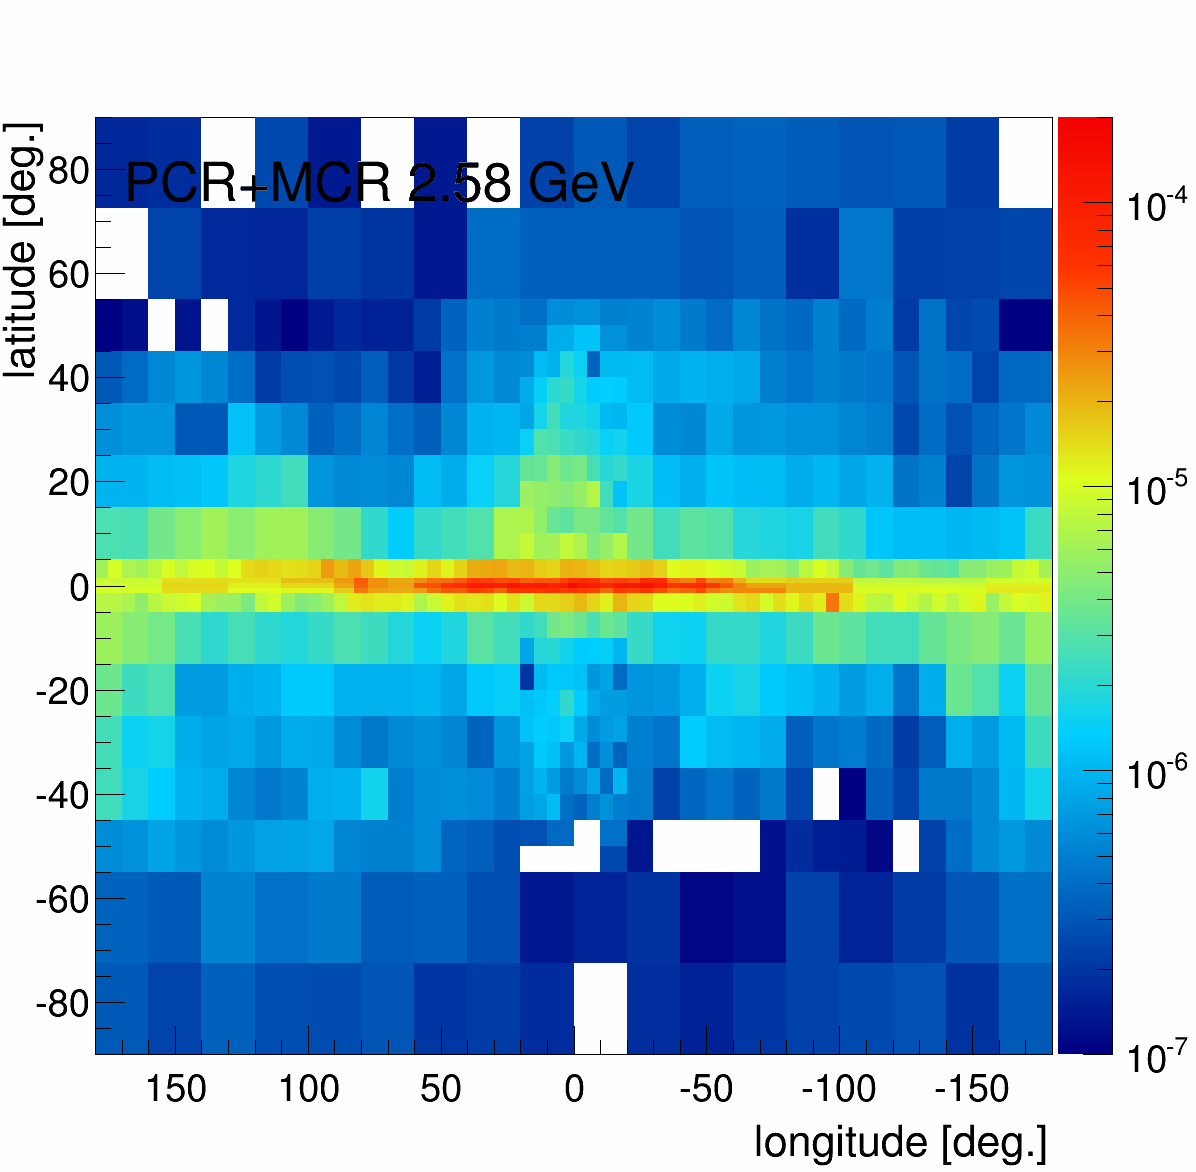
\includegraphics[width=1.\linewidth]{pic/results/MCRonly_PCR+MCR_fluxE12_skymap.png}
%  	\subcaption{Flux distribution of PCR + MCR}
%  	\label{fig:MCRonly_skymap_PCR+MCR}
%  \end{minipage}
%  \caption{}
%  \label{fig:MCRonly_skymaps}
%\end{figure}












